\documentclass[12pt]{article}

\usepackage{packages}
\usepackage{tabularx}
\usepackage{multirow}
\usepackage{graphicx}
\usepackage{float}
\usepackage{import}
\usepackage{booktabs}
\usepackage{etoc}

% --- Biblatex med refsection for separate referanselister ---
\usepackage[backend=biber,
            style=authoryear,
            maxcitenames=2,
            urldate=long,
            refsection=chapter
           ]{biblatex}
\addbibresource{Oppgave1/references.bib}
\addbibresource{Oppgave2/references.bib}
\addbibresource{Oppgave3/references.bib}
\addbibresource{Oppgave4/references.bib}
\addbibresource{Oppgave5/references.bib}

% --- Usynlig rapportnivå for etoc-scoping ---
% Gir hver rapport sin egen innholdsfortegnelse, figurliste og tabelliste
\newcounter{report}
\makeatletter
\newcommand{\l@report}[2]{} % Ikke vis rapportnivået i noen lister
\makeatother
\etocsetlevel{report}{-2}   % Høyere enn \part (-1)

\newcommand{\reportstart}{%
  \stepcounter{report}%
  % Legg inn usynlige skillemerker i toc/lof/lot for etoc-scoping
  \addtocontents{toc}{\protect\contentsline{report}{}{}{}}%
  \addtocontents{lof}{\protect\contentsline{report}{}{}{}}%
  \addtocontents{lot}{\protect\contentsline{report}{}{}{}}%
  % Nullstill alle tellere for ny selvstendig rapport
  \setcounter{section}{0}%
  \setcounter{subsection}{0}%
  \setcounter{subsubsection}{0}%
  \setcounter{figure}{0}%
  \setcounter{table}{0}%
  \setcounter{equation}{0}%
  \setcounter{footnote}{0}%
  \setcounter{part}{0}%
}

\begin{document}

% ============================================================
%  OPPGAVE 1: Kvile AS
% ============================================================
\reportstart
\begin{refsection}[Oppgave1/references.bib]

\begin{titlepage}
\vbox{ }
\vbox{ }
\begin{center}

\includegraphics[width=0.40\textwidth]{NTNU_logo.png}\\[1cm]
\textsc{\Large MAST1102 - Maskinteknikk 2}\\[0.5cm]
\textsc{\Large Industriell Drift og Vedlikehold}\\[0.5cm]
\vbox{ }
\HRule \\[0.4cm]
{ \huge \bfseries Rapport 1: Kvile AS}\\[0.4cm]
\HRule \\[1.5cm]
\large
\emph{Kandidatnummer:}\\
\vfill
{\large Dato 08/05/2026 }
\end{center}
\end{titlepage}

\frontmatter

\newpage
\section*{Sammendrag}
Rapporten vurderer hvordan Kvile AS bør styre produksjon, layout og bærekraftstiltak gitt dagens kundemiks. Kvile produserer utemøbler i aluminium og tre for Statens vegvesen, Plantasjen og Møbelringen, og rapporten besvarer fire deloppgaver knyttet til marked, produksjonsstyring, layout og bærekraft.

Kvile klassifiseres som en serie- og batchprodusent med over 300 produktvarianter og en omsetning på ca.\ 200 MNOK. Etterspørselen er sterkt sesongavhengig, med en topp i sommermånedene. Hovedanbefalingen er at Kvile viderefører ordreproduksjon (MTO) for Vegvesenet, men endrer styringen av butikkmarkedet fra produksjon til lager (MTS) til montasje på ordre (ATO). Dette flytter kundeordrens dekoblingspunkt til komponentlageret og reduserer antall lagervarer med ca.\ 76\,\%.

Fabrikklayouten vurderes som primært funksjonell, med linjeorganiserte lakkanlegg. Bærekraftsanalysen identifiserer forbedringsmuligheter innen emballasje, materialvalg, transport og produktdesign.

\newpage
\localtableofcontents
\locallistoffigures
\locallistoftables

\mainmatter

\newpage
\section*{Innledning}
\addcontentsline{toc}{section}{Innledning}

Denne rapporten analyserer produksjonsbedriften Kvile AS i deloppgave 1 i MAST1102 Maskinteknikk 2. Kvile produserer utemøbler i aluminium og tre i Orkanger, og leverer til Statens vegvesen, Plantasjen og Møbelringen. Rapporten vurderer marked og produkter, produksjonsstyring, layout og bærekraft, før hovedfunnene oppsummeres i en samlet konklusjon.
\section*{Oppgave 1 - Beskrivelse av produktene, markedet og kundene}
\setcounter{section}{1}
\setcounter{subsection}{0}
\addcontentsline{toc}{section}{Oppgave 1 — Markedsmiks}


\subsection{Analyse av Kviles markedssegmentering}
Kvile AS produserer robuste møbler til utendørs bruk. Høy variantbredde øker kompleksiteten i produksjon og lagerstyring, særlig når etterspørselen er sesongpreget \parencite{strandhagen2024}. Møblene produseres i Orkanger, Trøndelag, og distribueres til hele Norge. Denne seksjonen analyserer Kviles marked, kundesegmenter, produktmiks og etterspørselsmønster. Caset tar utgangspunkt i situasjonen per 1.\ november 2024.

\textbf{Kundegruppen}\\
Selskapet har tre store kunder: Statens Vegvesen, Plantasjen og Møbelringen. Vegvesenet er den største kunden målt i omsetning med 125 millioner kroner i årlig salgsvolum, mot 75 millioner til Plantasjen og Møbelringen. Vegvesenet står dermed for ca.\ 63\,\% av omsetningen, selv om antall enheter er likt (omtrent 15\,000 møbler til begge grupper). Vegvesenet betaler altså mye mer per møbel enn butikkene: 8\,333 kr (inkl.\ transport og montering på rasteplass) mot 5\,000 NOK.

\textbf{Produktmiks}\\
Kvile har fem produktserier: RAST, KVIL, KOS, KLEM og TRE. Produktvariasjonen skyldes kombinasjoner av modell, materialvalg, farge på aluminium, farge på treverk og type møbel (bord/benk). Som vist i tabell~\ref{tab:produktvarianter}, gir dette 308 SKU-er (Stock Keeping Unit) i 2024, med en økning på 96 SKU-er for hver nye aluminiumsmodell.

\begin{table}[htbp]
    \centering
    \caption[Produktvarianter per 2024]{Produktvarianter hos Kvile AS per 2024.}
    \label{tab:produktvarianter}
    \small
    \begin{tabular}{@{}lcccc@{}}
        \toprule
        \textbf{Modell} & \textbf{Alu} & \textbf{Tre} & \textbf{Typer} & \textbf{SKU-er} \\
                         & \textbf{farger} & \textbf{farger} & (bord+benk) & \\
        \midrule
        RAST (alu+tre) & 2  & 1 & 2 & 4   \\
        KVIL (alu+tre) & 6  & 8 & 2 & 96  \\
        KOS (alu+tre)  & 6  & 8 & 2 & 96  \\
        KLEM (alu+tre) & 6  & 8 & 2 & 96  \\
        TRE (kun tre)  & -- & 8 & 2 & 16  \\
        \midrule
        \multicolumn{4}{@{}l}{\textbf{Totalt 2024}} & \textbf{308} \\
        \multicolumn{4}{@{}l}{\textit{Etter ny modell 2025}} & \textit{404} \\
        \multicolumn{4}{@{}l}{\textit{Etter ny modell 2026}} & \textit{500} \\
        \bottomrule
    \end{tabular}
    
    \vspace{4pt}
    \raggedright\footnotesize
    \textit{Merk:} SKU = alu-farger $\times$ tre-farger $\times$ 2 (bord/benk). Ny aluminiummodell hvert år gir $+96$ varianter.
\end{table}

Kvile produserer rundt 30\,000 møbler i året fordelt på 308 unike produktvarianter. Volumet er for høyt til å klassifiseres som stykkproduksjon, men variasjonen gjør masseproduksjon uaktuelt. Betydelig omstillingstid på lakkanleggene gjør at Kvile må samle opp produksjon i serier av samme farge. Dette er kjennetegnet på serie-/batchproduksjon: middels volum kombinert med middels variasjon \parencite{slack2019}. Figur~\ref{fig:volum-variasjon} viser hvor Kvile plasseres i volum-variasjonsmatrisen.


% FIGUR 1: Volum vs. variasjon-matrisen

\begin{figure}[htbp]
    \centering
    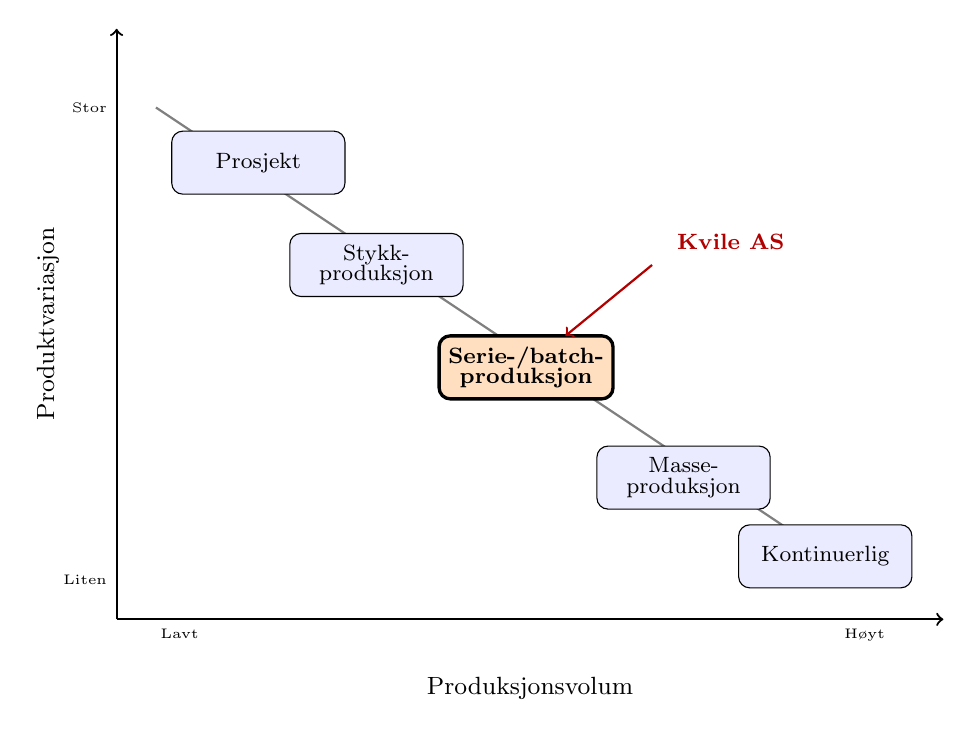
\begin{tikzpicture}[scale=1.0]
        % Akser
        \draw[->, thick] (0,0) -- (10.5,0) node[below, midway, yshift=-0.6cm, font=\small] {Produksjonsvolum};
        \draw[->, thick] (0,0) -- (0,7.5) node[above, rotate=90, midway, xshift=0cm, yshift=0.6cm, font=\small] {Produktvariasjon};
        
        % Diagonal linje
        \draw[thick, black!50] (0.5,6.5) -- (9.5,0.5);
        
        % Prosesstyper som bokser langs diagonalen
        \node[draw, rounded corners, fill=blue!8, minimum width=2.2cm, minimum height=0.8cm, font=\footnotesize] 
            at (1.8, 5.8) {Prosjekt};
        \node[draw, rounded corners, fill=blue!8, minimum width=2.2cm, minimum height=0.8cm, font=\footnotesize, align=center] 
            at (3.3, 4.5) {Stykk-\\[-2pt]produksjon};
        \node[draw, rounded corners, fill=orange!25, line width=1.2pt, minimum width=2.2cm, minimum height=0.8cm, font=\footnotesize\bfseries, align=center] 
            at (5.2, 3.2) {Serie-/batch-\\[-2pt]produksjon};
        \node[draw, rounded corners, fill=blue!8, minimum width=2.2cm, minimum height=0.8cm, font=\footnotesize, align=center] 
            at (7.2, 1.8) {Masse-\\[-2pt]produksjon};
        \node[draw, rounded corners, fill=blue!8, minimum width=2.2cm, minimum height=0.8cm, font=\footnotesize] 
            at (9.0, 0.8) {Kontinuerlig};
        
        % Kvile-markør
        \draw[->, thick, red!70!black] (6.8, 4.5) -- (5.7, 3.6);
        \node[font=\footnotesize\bfseries, red!70!black, align=center] at (7.8, 4.8) {Kvile AS};
        
        % Akselabels
        \node[font=\tiny, anchor=east] at (0, 6.5) {Stor};
        \node[font=\tiny, anchor=east] at (0, 0.5) {Liten};
        \node[font=\tiny, anchor=north] at (0.8, 0) {Lavt};
        \node[font=\tiny, anchor=north] at (9.5, 0) {Høyt};
    \end{tikzpicture}
    \caption[Volum vs.\ variasjon]{Prosesstyper: volum vs.\ variasjon. Kvile plasseres i serie-/batchproduksjon med middels volum ($\sim$30\,000 enheter/år) og middels-høy variasjon (308+ varianter). Basert på Slack \& Brandon-Jones (2019).}
    \label{fig:volum-variasjon}
\end{figure}


\textbf{Etterspørsel}\\
Etterspørselen etter Kviles produkter er preget av store sesongsvingninger, noe som er naturlig gitt at bedriften utelukkende produserer utemøbler for det norske markedet. Figur~\ref{fig:ettersporselsfordeling} illustrerer den estimerte månedlige etterspørselen fordelt på de to kundesegmentene. Vegvesenets leveranser er ordrestyrt (MTO). Bestillingene kommer minst fire måneder i forveien og gir Kvile et forutsigbart produksjonsgrunnlag, men leveransene tas kun imot i perioden mars til november. Butikkmarkedet er derimot lagerstyrt (MTS): Plantasjen og Møbelringen forventer at ferdigvarer er tilgjengelige til enhver tid, og etterspørselen fordeler seg over hele året. Likevel er det en markant sesongtopp, ettersom 50\,\% av butikksalget skjer i mai, juni og juli. Samlet gir dette en tydelig etterspørselstopp i sommermånedene, som vist i figur~\ref{fig:ettersporselsfordeling}. Det er denne sesongtoppen som gjør planleggingen vanskelig: enten må Kvile bygge opp lager gjennom lavsesongen, eller så må kapasiteten dimensjoneres for toppbelastning med mye ledig kapasitet resten av året.


% FIGUR 2: Årlig etterspørselskurve per måned (stacked)

\begin{figure}[htbp]
    \centering
    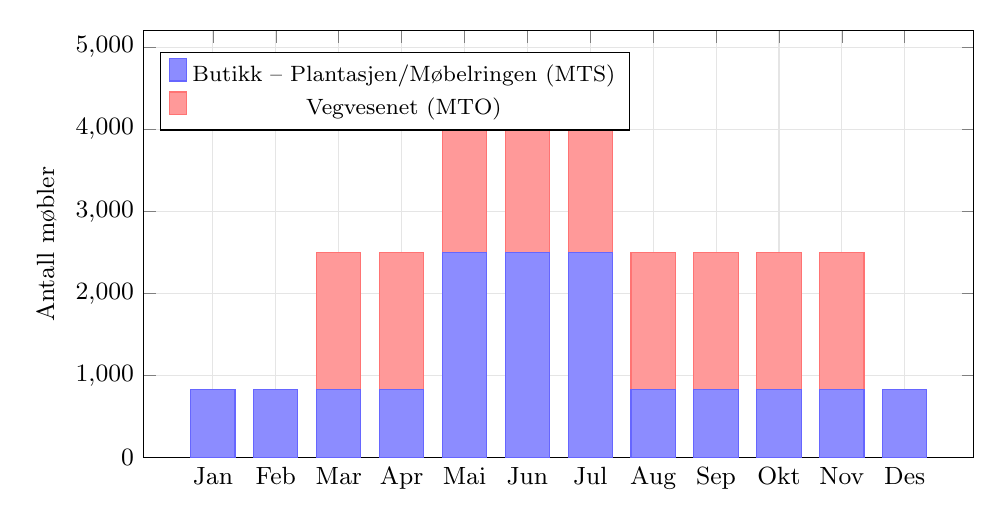
\begin{tikzpicture}
    \begin{axis}[
        width=\textwidth, height=7cm,
        ybar stacked,
        bar width=16pt,
        ymin=0, ymax=5200,
        ylabel={Antall møbler},
        symbolic x coords={Jan,Feb,Mar,Apr,Mai,Jun,Jul,Aug,Sep,Okt,Nov,Des},
        xtick=data,
        x tick label style={font=\small},
        y tick label style={font=\small},
        ylabel style={font=\small},
        legend style={at={(0.02,0.95)}, anchor=north west, font=\footnotesize},
        grid=major,
        grid style={gray!20},
    ]
    
    % Bunn: Plantasjen/Møbelringen (MTS)
    \addplot[fill=blue!45, draw=blue!60] coordinates {
        (Jan, 833)
        (Feb, 833)
        (Mar, 833)
        (Apr, 833)
        (Mai, 2500)
        (Jun, 2500)
        (Jul, 2500)
        (Aug, 833)
        (Sep, 833)
        (Okt, 833)
        (Nov, 833)
        (Des, 833)
    };
    
    % Topp: Vegvesenet (MTO)
    \addplot[fill=red!40, draw=red!55] coordinates {
        (Jan, 0)
        (Feb, 0)
        (Mar, 1667)
        (Apr, 1667)
        (Mai, 1667)
        (Jun, 1667)
        (Jul, 1667)
        (Aug, 1667)
        (Sep, 1667)
        (Okt, 1667)
        (Nov, 1667)
        (Des, 0)
    };
    
    % Usynlig serie for å plassere total-labels over søylene
    \addplot[
        draw=none, fill=none,
        nodes near coords={\pgfmathprintnumber[fixed, precision=0]{\pgfplotspointmeta}},
        nodes near coords style={font=\tiny\bfseries, anchor=south, yshift=1pt},
        point meta=explicit,
    ] coordinates {
        (Jan, 0)    [833]
        (Feb, 0)    [833]
        (Mar, 0)    [2500]
        (Apr, 0)    [2500]
        (Mai, 0)    [4167]
        (Jun, 0)    [4167]
        (Jul, 0)    [4167]
        (Aug, 0)    [2500]
        (Sep, 0)    [2500]
        (Okt, 0)    [2500]
        (Nov, 0)    [2500]
        (Des, 0)    [833]
    };
    
    \legend{Butikk -- Plantasjen/Møbelringen (MTS), Vegvesenet (MTO)}
    \end{axis}
    \end{tikzpicture}
    \caption[Månedlig etterspørsel]{Estimert total månedlig etterspørsel for Kvile AS (2023-tall). Tallene over søylene viser samlet etterspørsel fra begge segmenter. Totalvolum: $\sim$30\,000 møbler per år.}
    \label{fig:ettersporselsfordeling}
\end{figure}



\section*{Oppgave 2 - Produksjonsstyring}
\setcounter{section}{2}
\addcontentsline{toc}{section}{Oppgave 2 — Produksjonsstyring}

\setcounter{subsection}{0}
\subsection{Relevant teori}
Kundeordrens dekoblingspunkt (KODP) er det punktet i materialflyten som skiller produksjon basert på kundeordre fra produksjon basert på prognose eller lagernivå \parencite{strandhagen2024}. Plasseringen av KODP gir opphav til fire hovedstyringsformer: engineering på ordre (ETO), produksjon på ordre (MTO), montasje på ordre (ATO) og produksjon til lager (MTS). Når KODP ligger langt oppstrøms, slik som ved MTO, skjer en større del av produksjonen etter kundeordre. Det gir høy fleksibilitet, men lengre leveringstid. Når KODP ligger langt nedstrøms, slik som ved MTS, produseres mer på prognose, noe som gir kort leveringstid men øker risikoen for feil lagerbeholdning \parencite{slack2019}.

I et trykksystem (push) styres produksjonen av prognoser, mens et sugsystem (pull) lar faktisk forbruk nedstrøms utløse påfyll \parencite{strandhagen2024}. Lean-filosofien vektlegger å redusere sløsing, blant annet overproduksjon, unødvendig lager og transport \parencite{strandhagen2024}.


\subsection{Nåsituasjon hos Kvile}

Kvile bruker to ulike styringsformer. Vegvesenet styres som MTO, der produksjonen starter etter mottatt ordre. Butikksegmentet styres som MTS, der ferdig monterte og pakkede produkter ligger på ferdigvarelager. Forskjellene er oppsummert i tabell~\ref{tab:styringsformer} og illustrert i figur~\ref{fig:kodp}.

Begge segmentene benytter i praksis et trykksystem (push): for Vegvesenet trykkes produksjonen gjennom fabrikken av kundeordren, mens butikksegmentet trykkes av salgsprognoser. Produksjonen foregår i serier/batcher, der farge dikterer seriestørrelsen da betydelig omstillingstid på lakkanleggene gjør det nødvendig å samle opp produksjon av samme farge.

Sett i et Lean-perspektiv har Kviles nåværende oppsett potensielt flere former for sløsing: \textit{overproduksjon} av fargekombinasjoner med lavt salg (MTS med 304 SKU-er), \textit{unødvendig lager} bundet i ferdigvarer, \textit{venting} grunnet to døgns tørketid etter lakkering, og \textit{transport} med 10 lastebiler i tre-dagers turer gjennom hele Norge.

% --- Tabell: Styringsformer ---
\begin{table}[htbp]
    \centering
    \caption[Styringsformer]{Sammenligning av styringsformer hos Kvile AS.}
    \label{tab:styringsformer}
    \small
    \begin{tabular}{@{}lll@{}}
        \toprule
        & \textbf{Vegvesenet} & \textbf{Plantasjen/Møbelringen} \\
        \midrule
        Styringsform        & MTO                & MTS \\
        KODP                & Råvarelager         & Ferdigvarelager \\
        Styringsprinsipp    & Push (kundeordre)   & Push (prognose) \\
        Antall varianter    & 4                   & 304 \\
        Leveringstid        & $\geq$ 4 måneder   & Fra lager \\
        Planleggingshorisont & Lang, forutsigbar  & Kort, usikker \\
        \bottomrule
    \end{tabular}
\end{table}


\subsection{Vurdering og endringsforslag}

MTO-styringen av Vegvesenet er godt tilpasset både kundens og Kviles behov. Lang ordrehorisont, lavt antall varianter og forutsigbar etterspørsel gjør at Kvile kan planlegge kapasiteten effektivt uten å binde kapital i ferdigvarer. Denne styringsformen bør videreføres.

MTS-styringen for butikkmarkedet er derimot utfordrende. Med 304 varianter på ferdigvarelager blir kapitalbindingen stor, og risikoen for å sitte igjen med fargekombinasjoner som ikke selger er reell. Sesongsvingningene forsterker problemet — 50\,\% av salget skjer i mai--juli, noe som krever enten stor lageroppbygging i forkant eller kraftig kapasitetsøkning om våren. I tillegg vokser variantantallet med 96 nye SKU-er for hver ny modell.

\textbf{Forslag: Overgang til montasje på ordre (ATO).} Kvile kan flytte KODP fra ferdigvarelageret til komponentlageret ved å lagre ferdige, lakkerte halvfabrikata slik som aluminiumsrammer og trekomponenter separat. Når en ordre fra Plantasjen eller Møbelringen mottas, monteres riktig kombinasjon av ramme og tredeler, pakkes og klargjøres for henting. Dette er praktisk gjennomførbart fordi sluttmontasjen ifølge casebeskrivelsen kun krever enkle verktøy som skrutrekker og skiftenøkkel, og kjedene har tilstrekkelig ledetid (Plantasjen bestiller annenhver uke, Møbelringen månedlig).

Effekten på lagerkompleksiteten er stor. Tabell~\ref{tab:ato-sammenligning} viser hvordan antall lagervarer reduseres ved en overgang fra MTS til ATO.

% --- Tabell: MTS vs ATO lagervarer ---
\begin{table}[htbp]
    \centering
    \caption[MTS vs.\ ATO lagervarer]{Sammenligning av antall lagervarer (SKU-er) ved MTS og ATO for butikkmarkedet.}
    \label{tab:ato-sammenligning}
    \small
    \begin{tabular}{@{}lcc@{}}
        \toprule
        & \textbf{MTS (nå)} & \textbf{ATO (forslag)} \\
        \midrule
        Alu-rammer (4 modeller $\times$ 6 farger $\times$ delsett)
            & --- & $\sim$48 \\
        Trekomponenter (8 farger $\times$ delsett)
            & --- & $\sim$24 \\
        Ferdigvarer (bord + benk, alle kombinasjoner)
            & 304 & 0 \\
        \midrule
        \textbf{Totalt på lager} & \textbf{304} & $\mathbf{\sim}$\textbf{72} \\
        \textbf{Reduksjon} & & \textbf{$\sim$76\,\%} \\
        \bottomrule
    \end{tabular}
\end{table}

I tillegg bør Kvile vurdere å redusere farger med lav omløpshastighet og innføre syklisk styring av lakkanleggene.

% FIGUR: Kundeordrens dekoblingspunkt (KODP) hos Kvile AS


\begin{figure}[htbp]
    \centering
    \begin{tikzpicture}[
        node distance=0.5cm and 0.55cm,
        box/.style={draw, rounded corners=2pt, minimum height=0.75cm, minimum width=1.4cm, font=\scriptsize, align=center},
        progbox/.style={box, fill=gray!20},
        ordrebox/.style={box, fill=orange!20},
        arrw/.style={-{Stealth[length=2mm]}, semithick},
        lbl/.style={font=\tiny, text=black!55},
        >={Stealth[length=2mm]},
    ]

    % ===== VEGVESENET (MTO) =====
    \node[font=\scriptsize\bfseries, anchor=east] at (-0.3, 0) {Vegvesenet};
    \node[font=\tiny, anchor=east, text=black!50] at (-0.3, -0.3) {(MTO)};

    \node[progbox]  (v-inn)   at (1.0, 0) {Innkjøp};
    \node[ordrebox, right=of v-inn]  (v-prod) {Produksjon};
    \node[ordrebox, right=of v-prod] (v-mont) {Montasje};
    \node[ordrebox, right=of v-mont] (v-lev)  {Levering};
    \node[box, right=of v-lev, fill=blue!10]  (v-kunde) {Kunde};

    \draw[arrw] (v-inn) -- (v-prod);
    \draw[arrw] (v-prod) -- (v-mont);
    \draw[arrw] (v-mont) -- (v-lev);
    \draw[arrw] (v-lev) -- (v-kunde);

    % KODP
    \coordinate (v-kodp) at ($(v-inn.east)!0.5!(v-prod.west)$);
    \draw[red!70!black, thick, dashed] (v-kodp) ++(0, 0.55) -- ++(0, -1.1);
    \node[font=\tiny\bfseries, red!70!black, above] at ($(v-kodp)+(0, 0.55)$) {KODP};

    \node[lbl] at ($(v-inn)+(0, 0.6)$) {Prognose};
    \node[lbl] at ($(v-prod)+(0, 0.6)$) {Kundeordre};


    % ===== BUTIKK NÅ (MTS) =====
    \node[font=\scriptsize\bfseries, anchor=east] at (-0.3, -2.2) {Butikk \textit{(nå)}};
    \node[font=\tiny, anchor=east, text=black!50] at (-0.3, -2.5) {(MTS)};

    \node[progbox] (b-inn)   at (1.0, -2.2) {Innkjøp};
    \node[progbox, right=of b-inn]  (b-prod)  {Produksjon};
    \node[progbox, right=of b-prod] (b-mont)  {Montasje};
    \node[progbox, right=of b-mont] (b-lager) {FV-lager};
    \node[box, right=of b-lager, fill=blue!10] (b-kunde) {Kunde};

    \draw[arrw] (b-inn)  -- (b-prod);
    \draw[arrw] (b-prod) -- (b-mont);
    \draw[arrw] (b-mont) -- (b-lager);
    \draw[arrw] (b-lager) -- (b-kunde);

    % KODP
    \coordinate (b-kodp) at ($(b-lager.east)!0.5!(b-kunde.west)$);
    \draw[red!70!black, thick, dashed] (b-kodp) ++(0, 0.55) -- ++(0, -1.1);
    \node[font=\tiny\bfseries, red!70!black, above] at ($(b-kodp)+(0, 0.55)$) {KODP};

    \node[lbl] at ($(b-inn)+(0, 0.6)$) {Prognose};
    \node[lbl] at ($(b-mont)+(0, 0.6)$) {Prognose};

    % 304 SKU-er
    \node[font=\tiny, text=red!60!black, below=2pt of b-lager] {304 SKU-er};


    % ===== BUTIKK FORSLAG (ATO) =====
    \node[font=\scriptsize\bfseries, anchor=east] at (-0.3, -4.4) {Butikk \textit{(forslag)}};
    \node[font=\tiny, anchor=east, text=black!50] at (-0.3, -4.7) {(ATO)};

    \node[progbox] (a-inn)   at (1.0, -4.4) {Innkjøp};
    \node[progbox, right=of a-inn]  (a-prod)  {Prod.\ +\\[-2pt]lakk};
    \node[progbox, right=of a-prod] (a-lager) {Komp.-\\[-2pt]lager};
    \node[ordrebox, right=of a-lager] (a-mont) {Mont.\ +\\[-2pt]pakk};
    \node[box, right=of a-mont, fill=blue!10] (a-kunde) {Kunde};

    \draw[arrw] (a-inn)   -- (a-prod);
    \draw[arrw] (a-prod)  -- (a-lager);
    \draw[arrw] (a-lager) -- (a-mont);
    \draw[arrw] (a-mont)  -- (a-kunde);

    % KODP
    \coordinate (a-kodp) at ($(a-lager.east)!0.5!(a-mont.west)$);
    \draw[red!70!black, thick, dashed] (a-kodp) ++(0, 0.55) -- ++(0, -1.1);
    \node[font=\tiny\bfseries, red!70!black, above] at ($(a-kodp)+(0, 0.55)$) {KODP};

    \node[lbl] at ($(a-inn)+(0, 0.6)$) {Prognose};
    \node[lbl] at ($(a-mont)+(0, 0.6)$) {Kundeordre};

    % ~72 SKU-er
    \node[font=\tiny, text=green!50!black, below=2pt of a-lager] {$\sim$72 SKU-er};


    % ===== FORKLARING =====
    \node[draw, rounded corners, fill=white, inner sep=4pt, font=\tiny, anchor=north west] 
        at (-0.3, -5.8) {%
            \textcolor{gray!50}{\rule{0.4cm}{4pt}} Prognosestyrt \quad
            \textcolor{orange!45}{\rule{0.4cm}{4pt}} Ordrestyrt \quad
            \textcolor{red!70!black}{- - -} KODP
        };

    \end{tikzpicture}
    \caption[KODP for Kviles kundesegmenter]{Kundeordrens dekoblingspunkt (KODP) for Kviles to kundesegmenter. Øverst: Vegvesenet (MTO). Midten: butikkmarkedet i dag (MTS) med 304 SKU-er på ferdigvarelager. Nederst: foreslått ATO-løsning med $\sim$72 komponent-SKU-er.}
    \label{fig:kodp}
\end{figure}
\section*{Oppgave 3 - Layout}
\setcounter{section}{3}
\addcontentsline{toc}{section}{Oppgave 3 — Layout}

\setcounter{subsection}{0}

\subsection{Kviles layout}

Layout beskriver hvordan produksjonsressurser er fysisk plassert i fabrikken \parencite{strandhagen2024}. Hovedskillet går mellom \textit{funksjonell layout} (gruppert etter prosesstype) og \textit{linje-/produktlayout} (fast rekkefølge) \parencite{slack2019}.

Produksjonen hos Kvile består av aluminiumbearbeiding, snekkeravdeling, trekomponentmontasje, lakkering (to separate anlegg med betydelig omstillingstid), tørking, endemontering og pakking. Ulike produkter følger ulike ruter: rene treprodukter hopper over aluminiumbearbeiding, mens aluminium/tre-modellene behandles i parallell gjennom begge materialløpene før de møtes i endemonteringen. Dette samsvarer med \textit{funksjonell layout}: ressurser gruppert etter prosesstype, og produktene flyttes mellom avdelingene etter behov.

Lakkeanleggene har imidlertid trekk av \textit{linjelayout} internt, da alle deler følger samme sekvens (forbehandling $\rightarrow$ lakkering $\rightarrow$ tørking). Kviles layout kan dermed beskrives som en \textbf{kombinasjon}: primært funksjonell layout på fabrikknivå, med linjeorganiserte lakkeanlegg som delte ressurser. Figur~\ref{fig:layout-flyt} illustrerer materialflyten gjennom fabrikken.

Dersom Kvile går over til ATO for butikkmarkedet, som foreslått i oppgave~2, bør layouten også tilpasses. Komponentlageret bør plasseres nær endemontering og pakking, slik at sluttmontasjen kan gjennomføres med kort gjennomløpstid. Dette vil redusere intern transport og gjøre det enklere å styre montasjen etter faktiske kundeordrer.

\begin{figure}[htbp]
    \centering
    \begin{tikzpicture}[
        node distance=1.1cm,
        block/.style={rectangle, draw, rounded corners, minimum width=2.8cm, minimum height=0.85cm, align=center, font=\small},
        alu/.style={block, fill=blue!12},
        tre/.style={block, fill=green!12},
        felles/.style={block, fill=orange!15},
        arr/.style={-{Stealth[length=2.5mm]}, thick},
    ]
        % --- Venstre kolonne: Aluminium ---
        \node[alu] (alu-raw) {Aluminium (råvare)};
        \node[alu, below=of alu-raw] (alu-bearb) {Al-bearbeiding\\{\footnotesize kapp/bøy/slip/vask}};
        \node[alu, below=of alu-bearb] (alu-lakk) {Lakkering Al\\+ tørking (2 døgn)};
 
        % --- Høyre kolonne: Tre ---
        \node[tre, right=2.5cm of alu-raw] (tre-raw) {Treverk (råvare)};
        \node[tre, below=of tre-raw] (tre-bearb) {Snekkeravd.\\{\footnotesize kapp/fres/slip}};
        \node[tre, below=of tre-bearb] (tre-mont) {Trekomp.-montasje\\{\footnotesize plate/sete/rygg}};
        \node[tre, below=of tre-mont] (tre-lakk) {Lakkering tre\\+ tørking (2 døgn)};
 
        % --- Felles bunn ---
        \node[felles, below=1.3cm of $(alu-lakk)!0.5!(tre-lakk)$] (ende) {Endemontering};
        \node[felles, below=of ende] (pakk) {Pakking / lager};
 
        % Piler aluminium (ned)
        \draw[arr, blue!60] (alu-raw) -- (alu-bearb);
        \draw[arr, blue!60] (alu-bearb) -- (alu-lakk);
        \draw[arr, blue!60] (alu-lakk) |- (ende);
 
        % Piler tre (ned)
        \draw[arr, green!50!black] (tre-raw) -- (tre-bearb);
        \draw[arr, green!50!black] (tre-bearb) -- (tre-mont);
        \draw[arr, green!50!black] (tre-mont) -- (tre-lakk);
        \draw[arr, green!50!black] (tre-lakk) |- (ende);
 
        % Endemontering til pakking
        \draw[arr] (ende) -- (pakk);
 
        % Kolonne-labels
        \node[above=0.3cm of alu-raw, font=\footnotesize\bfseries, blue!70] {Aluminiumløp};
        \node[above=0.3cm of tre-raw, font=\footnotesize\bfseries, green!50!black] {Treløp};
 
    \end{tikzpicture}
    \caption[Materialflyt hos Kvile AS]{Materialflyt hos Kvile AS. Blått løp viser aluminiumbearbeiding, grønt løp viser trebearbeiding. De to løpene møtes i endemonteringen. Layouten er primært funksjonell, med linjeorganiserte lakkeanlegg.}
    \label{fig:layout-flyt}
\end{figure}
\section*{Oppgave 4 — Bærekraft}
\setcounter{section}{4}
\addcontentsline{toc}{section}{Oppgave 4 — Bærekraft}

\setcounter{subsection}{0}

\subsection{Kviles bærekraft}

\textbf{Økonomisk} har Kvile et godt utgangspunkt med ca.\ 200~MNOK i omsetning, vekst og en stabil offentlig kunde. \textbf{Sosialt} bidrar bedriften med industriarbeidsplasser i Orkanger og møbler til offentlige rasteplasser. \textbf{Miljømessig} er vurderingen svakere: aluminium er energikrevende, lakkering kan gi kjemikalie- og VOC-utslipp, transporten skjer med lastebil over hele Norge, og RAST-produktene bruker engangsemballasje av glassfiberstrie.

\subsection{Endringsforslag}

Det mest åpenbare tiltaket gjelder emballasjen. Glassfiberstrien rundt RAST-produktene er en ren engangsløsning som kastes ved montering. Kvile bør heller utvikle returemballasje — f.eks.\ vevde tekstilposer eller stålrammer — som sjåførene tar med tilbake etter levering. Siden Kviles egen transportavdeling utfører leveransene, er returlogistikken allerede på plass.

Kvile bør også gå over til resirkulert aluminium, som krever ca.\ 95\,\% mindre energi enn primæraluminium \parencite{iai2025}.

Når det gjelder transport og produktdesign ser vi to muligheter. Fabrikken ligger nær kaia på Orkanger, men Kvile bruker utelukkende lastebil. For leveranser til kystbyer kan sjøtransport kombinert med lokal distribusjon redusere utslipp, og ruteoptimalisering av lastebilturene kan redusere tomkjøring. Samtidig bør Kvile designe produktene slik at slitedeler som treplatene kan skiftes uten å bytte hele møbelet. Dette er spesielt relevant for Vegvesenet, som i dag bestiller komplette erstatninger for slitte møbler.

Flere av disse tiltakene henger sammen med Lean-prinsippene fra oppgave~2. ATO reduserer overproduksjon og unødvendig lager, returemballasje kutter materialavfall, og bedre ruter betyr mindre transportsløsing.
\section*{Konklusjon}
\addcontentsline{toc}{section}{Konklusjon}

Kvile AS er en serie-/batchprodusent med høy variantbredde og tydelig sesongvariasjon. Dagens MTO-styring for Vegvesenet er hensiktsmessig og bør videreføres. Hovedanbefalingen er å flytte butikkmarkedets KODP fra ferdigvarelager til komponentlager gjennom ATO. Dette reduserer antall lagervarer med ca.\ 76\,\% og angriper hovedutfordringen: mange produktvarianter, sesongvariasjon og kapitalbinding i ferdigvarer.

Vi vurderer fabrikklayouten som primært funksjonell, med linjeorganiserte lakkanlegg. Ved overgang til ATO bør komponentlager plasseres nær endemontering og pakking. Bærekraften kan styrkes gjennom returemballasje, resirkulert aluminium, bedre ruteplanlegging og modulært design for reparasjon. Flere av tiltakene støtter også Lean-prinsipper ved å redusere lager, transport og materialavfall.


\newpage
\printbibliography[title={Referanser}]

\end{refsection}

% ============================================================
%  OPPGAVE 2: Lab Vibrasjon
% ============================================================
\reportstart
\begin{refsection}[Oppgave2/references.bib]

\newpage
\begin{titlepage}
\vbox{ }
\vbox{ }
\begin{center}

\includegraphics[width=0.40\textwidth]{NTNU_logo.png}\\[1cm]
\textsc{\Large MAST1102 - Maskinteknikk 2}\\[0.5cm]
\textsc{\Large Industriell Drift og Vedlikehold}\\[0.5cm]
\vbox{ }
\HRule \\[0.4cm]
{ \huge \bfseries Rapport 2: Lab Vibrasjon}\\[0.4cm]
\HRule \\[1.5cm]
\large
\emph{Kandidatnummer:}\\
\vfill
{\large Dato 08/05/2026 }
\end{center}
\end{titlepage}

\frontmatter

\newpage
\section*{Sammendrag}
I dette forsøket ble det gjennomført vibrasjonsmåling på et R10-kulelager montert i en Bently Nevada RK4-vibrasjonsrigg. Målingene ble gjort ved tre turtall (2498, 3998 og 6001 rpm) med piezoelektriske akselerometre koblet til SKF IMx-8, og analysert i SKF Observer.

Frekvensanalysen viste at de største utslagene kom ved grunnfrekvensen (1X), særlig ved 6001 rpm der amplituden nådde 2{,}239\,mm/s. Dette passer best med rotasjonsrelaterte vibrasjoner, for eksempel ubalanse. Amplitudene ved lagerfrekvensene for ytterring ($f_y$), innerring ($f_i$) og kule ($f_r$) var svært lave ved alle turtall. Målingene gir dermed ikke grunnlag for å påvise lokal lagerskade, og lageret vurderes til tilstandsgrad 1 med hensyn til lokal lagerskade.


\newpage
\localtableofcontents
\locallistoffigures
\locallistoftables

\mainmatter

\section{Innledning}
Vibrasjonsmåling er en vanlig metode for å følge med på tilstanden til roterende maskiner. Poenget er å oppdage endringer i vibrasjonsbildet før feilen utvikler seg til havari \parencite{vibrasjon1, tbv1}. Frekvensinnholdet i signalet kan gi informasjon om hvor vibrasjonen kommer fra, for eksempel om den skyldes ubalanse i akselen eller en lokal skade i lageret \parencite{nsen13306}. Vibrasjonsovervåking utnytter P-F-intervallet, altså tidsrommet mellom første detekterbare feil og funksjonssvikt, noe som gir mulighet til å planlegge vedlikehold i tide \parencite{tbv2}.

Formålet med denne laboratorieøvelsen er å måle vibrasjoner på et R10-kulelager montert i en RK4-vibrasjonsrigg, identifisere grunnfrekvensen og de karakteristiske lagerfrekvensene, og vurdere lagerets tilstand ut fra amplitudene i frekvensspekteret.

\section{Teori}

\subsection{Vibrasjonsmåling på kulelager}
Vibrasjoner i roterende maskiner skyldes ofte ubalanse, geometriske avvik, varierende belastning eller lokale skader i lageret \parencite{vibrasjon3}. I en slik analyse sier frekvensen mest om hvor vibrasjonen kommer fra, mens amplituden sier noe om hvor kraftig vibrasjonen er \parencite{vibrasjon1, vibrasjon2}.

Ubalanse gir typisk en tydelig topp ved grunnfrekvensen, også kalt 1X, fordi kraften opptrer én gang per omdreining \parencite{vibrasjon2}. Lokale skader i lageret gir derimot vibrasjoner ved karakteristiske lagerfrekvenser, avhengig av om skaden sitter i ytterring, innerring eller kule \parencite{vibrasjon3}.

\subsection{Forskyvning, hastighet og akselerasjon}
Vibrasjon kan beskrives som forskyvning, hastighet eller akselerasjon. Forskyvning egner seg best ved lave frekvenser, hastighet er mye brukt ved generell maskinvibrasjon, og akselerasjon fanger opp høyfrekvente signaler som ofte er knyttet til lagerfeil \parencite{vibrasjon1}. I dette forsøket ble vibrasjonene målt med akselerometre, mens resultatene vurderes som vibrasjonshastighet i mm/s.

\subsection{Overrullingsfrekvenser}
For å finne ut hvilken del av lageret som forårsaker vibrasjoner, kan målte frekvenser sammenlignes med de karakteristiske lagerfrekvensene \parencite{vibrasjon3, beregninglager}:
\begin{itemize}
    \item \textbf{BPFO} (Ball Pass Frequency Outer race), $f_y$ -- ytterringens overrullingsfrekvens
    \item \textbf{BPFI} (Ball Pass Frequency Inner race), $f_i$ -- innerringens overrullingsfrekvens
    \item \textbf{BSF} (Ball Spin Frequency), $f_r$ -- kulens rotasjonsfrekvens
\end{itemize}
I tillegg finnes FTF (Fundamental Train Frequency), som beskriver kuleholderens rotasjonsfrekvens, men denne analyseres ikke videre i forsøket.

Overrullingsfrekvensene kan beregnes fra lagergeometrien \parencite{beregninglager}:

\textbf{Overrullingsfrekvens ytterring (BPFO):}
\[
\text{BPFO} = \frac{N_B}{2} \left[ 1 - \frac{B_D}{P_D}\cos(\theta) \right] \cdot \frac{\text{RPM}}{60}
\]

\textbf{Overrullingsfrekvens innerring (BPFI):}
\[
\text{BPFI} = \frac{N_B}{2} \left[ 1 + \frac{B_D}{P_D}\cos(\theta) \right] \cdot \frac{\text{RPM}}{60}
\]

\textbf{Kulens rotasjonsfrekvens (BSF):}
\[
\text{BSF} = \frac{P_D}{2 B_D} \left[ 1 - \left( \frac{B_D}{P_D} \cos(\theta) \right)^2 \right] \cdot \frac{\text{RPM}}{60}
\]

Her er $N_B$ antall kuler, $B_D$ kulediameter, $P_D$ pitch diameter og $\theta$ kontaktvinkelen. For enradige kulelager som R10-lageret på BN-riggen kan kontaktvinkelen settes til $\theta = 0°$ \parencite{beregninglager}. I denne rapporten brukes frekvensene avlest fra SKF Observer videre i analysen. Formlene viser prinsippet bak lagerfrekvensene, men de endelige verdiene hentes fra måledataene.

\subsection{Lagerskader og frekvensspekter}
Lagerskader utvikler seg gradvis og gir ulike utslag i frekvensspekteret avhengig av skadegrad \parencite{vibrasjon3}. I tidlig fase oppstår små skader i kontaktflatene, noe som gir svake, høyfrekvente vibrasjoner. Disse signalene har ofte lav amplitude, som gjør at de ligger nært støygulvet og kan være vanskelige å identifisere. 
\newline Etter hvert som skaden utvikler seg, vil signalet gi tydeligere topper ved lagerfrekvensene, i henhold til hvor ofte lagerkulene passerer det skadde området.
\newline I praksis brukes frekvensspekteret til å identifisere slike mønstre. Tydelige topper ved $f_y$, $f_i$ eller $f_r$, indikerer lokal lagerskade. Fravær av slike topper betyr derimot ikke nødvendigvis at lageret er feilfritt, men at det ikke foreligger en utviklet skade som gir utslag i det målte frekvensområdet.
\newline I denne rapporten vurderes frekvensspekteret med fokus på om det finnes tydelige topper ved $f_y$, $f_i$ og $f_r$, som kan indikere skade i henholdsvis ytterring, innerring eller kule.
%Lagerskader utvikler seg gradvis \parencite{vibrasjon3}. Tidlige skader gir ofte høyfrekvente signaler, mens mer utviklede skader viser seg som tydelige topper ved lagerdefektfrekvensene og deres harmoniske. I denne rapporten ser vi etter om det finnes slike topper ved $f_y$, $f_i$ og $f_r$. Dersom slike topper ikke finnes, er det ikke grunnlag for å påvise en tydelig lokal lagerskade i målingen.

\subsection{Fourier-transformasjon}
Akselerometeret måler først vibrasjonen som et tidssignal. Dette signalet er vanskelig å tolke direkte, siden flere vibrasjonskilder kan opptre samtidig. Derfor omformes signalet til et frekvensspekter ved hjelp av Fourier-transformasjon \parencite{vibrasjon1}, slik at dominerende frekvenser kan identifiseres. Topper ved grunnfrekvensen kan peke mot ubalanse, mens topper ved lagerfrekvensene kan peke mot skader i ytterring, innerring eller kule.

\section{Metode}

\subsection{Målekjede}
Oppsettet følger en standard målekjede for tilstandsovervåking \parencite{tbv2}: vibrasjonen fanges opp av et akselerometer, sendes til en datainnsamlingsenhet (SKF IMx-8), og presenteres i analyseprogramvare (SKF Observer) der frekvensanalysen gjøres.

\subsection{Beskrivelse av oppstilling}
Forsøket ble gjennomført på en RK4-vibrasjonsrigg fra Bently Nevada. Riggen består av en DC-motor som driver en aksel opplagret i lagerbukker. Turtallet ble kontrollert og målt underveis, og vi kjørte målinger ved omtrent 2500, 4000 og 6000 rpm.

Vibrasjonene ble målt med piezoelektriske akselerometre fra SKF montert ved lageret \parencite{vibrasjon1}. Sensorene var koblet til ett SKF IMx-8 system, og signalene ble analysert i SKF Observer der vi leste av frekvenser og amplituder fra frekvensspekteret.

Sensorene ble plassert nær lageret for å redusere demping mellom lager og målepunkt \parencite{vibrasjon3}.

\subsubsection*{Lager brukt i forsøket}
I forsøket ble det brukt et R10-kulelager fra National Precision Bearing. Dette er et enradig kulelager med kontaktvinkel $\theta \approx 0°$ \parencite{beregninglager}.
\begin{table}[h!]
\centering
\begin{tabular}{|l|c|}
\hline
\textbf{Lagertype} & \textbf{Åpent rulle-/kulelager (R10)} \\ \hline
Antall kuler & 10 \\ \hline
Pitch diameter (mm) & 25.4 \\ \hline
Kulediameter (mm) & 4.7 \\ \hline
Indre diameter (mm) & 15.9 \\ \hline
Ytre diameter (mm) & 34.9 \\ \hline
\end{tabular}
\caption{Lagerdata for R10}
\end{table}

% TODO: Beskriv fremgangsmåte steg-for-steg (hvilke turtall, hvordan data ble hentet)
% TODO: Legg inn bilde av oppstillingen (fra øvingsarket eller eget foto)

\section{Resultater}

\subsection*{Førsteordens vibrasjon}
Grunnfrekvensen beregnes ved å konvertere turtallet fra rpm til Hz:
\[
f = \frac{\mathrm{RPM}}{60}
\]
Målingene skulle i utgangspunktet gjennomføres ved 2500, 4000 og 6000 rpm. Under laboratorieforsøket ble de faktiske turtallene målt til 2498, 3998 og 6001 rpm. Disse verdiene brukes videre i analysen.

\renewcommand{\arraystretch}{1.3}
\begin{table}[h]
\centering
\begin{tabular}{|c|c|}
\hline
Turtall (rpm) & Grunnfrekvens (Hz) \\
\hline
2498 & 42 \\
\hline
3998 & 67 \\
\hline
6001 & 100 \\
\hline
\end{tabular}
\caption{Grunnfrekvens for de målte turtallene}
\end{table}

\subsection*{Lagerfrekvensene $f_y$, $f_i$ og $f_r$}
Frekvensene $f_y$, $f_i$ og $f_r$ ble avlest fra SKF Observer for de tre turtallene.

\begin{table}[h]
\centering
\begin{tabular}{|c|c|c|c|}
\hline
Turtall (rpm) & $f_y$ (Hz) & $f_i$ (Hz) & $f_r$ (Hz) \\
\hline
2498 & 170 & 247 & 109 \\
\hline
3998 & 272 & 395 & 174 \\
\hline
6001 & 408 & 593 & 261 \\
\hline
\end{tabular}
\caption{Karakteristiske lagerfrekvenser for de målte turtallene}
\end{table}

\subsection*{Amplitude ved grunnfrekvens og lagerfrekvenser}
Amplitudene ved grunnfrekvensen og lagerfrekvensene ble avlest fra SKF Observer og er vist i tabell~\ref{tab:amplituder}.

\begin{table}[h]
\centering
\resizebox{0.6\textwidth}{!}{
\begin{tabular}{|c|c|c|c|c|}
\hline
Turtall (rpm) & $A(f)$ & $A(f_y)$ & $A(f_i)$ & $A(f_r)$ \\
\hline
2498 & 0.323 & 0.009 & 0.002 & 0.002 \\
\hline
3998 & 0.346 & 0 & 0 & 0 \\
\hline
6001 & 2.239 & 0.002 & 0.01 & 0.001 \\
\hline
\end{tabular}
}
\caption{Amplitude $A$ (mm/s) ved grunnfrekvens og lagerfrekvenser}
\label{tab:amplituder}
\end{table}

Amplituden er størst ved grunnfrekvensen $f$, mens amplitudene ved lagerfrekvensene $f_y$, $f_i$ og $f_r$ er svært små. Verdier oppgitt som null betyr at det ikke ble identifisert en tydelig topp ved den aktuelle frekvensen.

\section{Diskusjon}

\subsection{Tolkning av grunnfrekvensen}
Ved alle tre turtallene var det grunnfrekvensen som ga størst utslag. En dominerende 1X-topp passer med ubalanse eller lignende \parencite{vibrasjon2}. Amplituden økte merkbart fra 0{,}346\,mm/s ved 3998\,rpm til 2{,}239\,mm/s ved 6001\,rpm. Dette passer med at ubalansekrefter øker når turtallet øker \parencite{vibrasjon2}.

\subsection{Vurdering av lagerfrekvensene}
At lagerfrekvensene er lave, betyr ikke at alle mulige feil kan utelukkes. Vi finner likevel ikke grunnlag for å påvise lokale skader i ytterring, innerring eller kule \parencite{vibrasjon3}. De lave amplitudene ved lagerfrekvensene tilsier tilstandsgrad 1 med hensyn til lokal lagerskade \parencite{tbv2}.

\subsection{Vurdering etter ISO 10816}
Målingene kan sammenlignes indikativt med ISO 10816-3 for små maskiner, der grenseverdiene er 0{,}71\,mm/s, 1{,}80\,mm/s og 4{,}50\,mm/s \parencite{iso10816, vibrasjon1}. Ved 2498 og 3998\,rpm ligger amplitudene ved grunnfrekvensen i sone A, mens 6001\,rpm havner i sone C. Det er økningen ved grunnfrekvensen som drar opp verdien, ikke lagerfrekvensene. Sammenligningen må tolkes med forsiktighet, siden ISO-vurdering normalt bygger på samlet RMS-verdi og ikke enkeltamplituder ved bestemte frekvenser.

\subsection{Feilkilder}
Usikkerheten ligger først og fremst i målekjeden. Sensorplassering og innfesting kan påvirke hvor mye av vibrasjonen som faktisk fanges opp, særlig dersom signalet dempes mellom lageret og målepunktet \parencite{tbv2}. I tillegg kan bakgrunnsstøy fra riggen gjøre små topper vanskelige å skille fra støygulvet. Frekvensoppløsningen i FFT-analysen kan også ha påvirket hvor presist frekvenstoppene ble avlest.

Målingene er dessuten et øyeblikksbilde. I praksis bygger prediktivt vedlikehold på trendanalyse over tid, der endringer i vibrasjonsnivå over flere målinger gir et mer pålitelig bilde \parencite{vibrasjon2, tbv2}. Siden forsøket ble gjort på en kontrollert laboratorierigg, er typiske feilkilder som feilsmøring, forurensning og feilmontering mindre aktuelle her \parencite{vibrasjon3}.

% TODO: Legg inn frekvensspekter-figurer fra SKF Observer som støtter diskusjonen

\section{Konklusjon}
Målingene ved 2498, 3998 og 6001 rpm viste at den største vibrasjonen lå ved grunnfrekvensen. Økningen var særlig tydelig ved 6001 rpm, der amplituden nådde 2{,}239\,mm/s. Dette er forenlig med ubalanse eller andre rotasjonsrelaterte krefter, og er forventet for et normalt fungerende system.

Amplitudene ved lagerfrekvensene $f_y$, $f_i$ og $f_r$ var svært lave ved alle turtall. Forsøket gir derfor ingen tydelige indikasjoner på lokal skade i ytterring, innerring eller kule. De lave amplitudene tilsier tilstandsgrad 1 med hensyn til lokal lagerskade, og det anbefales å videreføre normal drift med periodisk vibrasjonsovervåking.


\newpage
\printbibliography[title={Referanser}]

\end{refsection}

% ============================================================
%  OPPGAVE 3: Tilstandsbasert Vedlikehold
% ============================================================
\reportstart
\begin{refsection}[Oppgave3/references.bib]

\newpage
\begin{titlepage}
\vbox{ }
\vbox{ }
\begin{center}

\includegraphics[width=0.40\textwidth]{NTNU_logo.png}\\[1cm]
\textsc{\Large MAST1102 - Maskinteknikk 2}\\[0.5cm]
\textsc{\Large Industriell Drift og Vedlikehold}\\[0.5cm]
\vbox{ }
\HRule \\[0.4cm]
{ \huge \bfseries Rapport 3: Tilstandsbasert Vedlikehold}\\[0.4cm]
\HRule \\[1.5cm]
\large
\emph{Kandidatnummer:}\\
\vfill
{\large Dato 08/05/2026 }
\end{center}
\end{titlepage}

\frontmatter

\newpage
\section*{Sammendrag}
Denne rapporten analyserer systempåliteligheten til et kompressortog for gassreinjisering på en oljeplattform. Kompressortoget består av en førstetrinns kompressor, en andretrinns kompressor og en elmotor, koblet i serie. Den beregnede systempåliteligheten er 76,1\%. Ved å innføre redundans på utvalgte komponenter kan påliteligheten økes til mellom 80\% og 98\%, avhengig av hvilke komponenter som parallellkobles. Rapporten anbefaler redundans på andretrinns kompressor og elmotor som et balansert tiltak, med en beregnet systempålitelighet på 92,9\%.

\newpage
\localtableofcontents
\locallistoftables

\mainmatter

\newpage
\newpage
\section{Innledning}
Rapporten vurderer systempåliteligheten til et kompressortog bestående av to kompressorer og én felles drivenhet, installert på en oljeplattform. Kompressorene benyttes til å komprimere gass for reinjisering i et reservoar. Systemet består av en førstetrinns kompressor, en andretrinns kompressor og en elmotor drevet av en gassturbin. For at kompressortoget skal fungere, må begge kompressorene og drivenheten være operative.

Først beregnes påliteligheten til eksisterende seriesystem. Deretter vurderes ulike redundansløsninger, og alternativene sammenlignes med hensyn til økt systempålitelighet, reparasjonstid og praktiske begrensninger.

\section{Teori}

Et seriesystem er et system der hver komponent må fungere for at systemet som helhet skal fungere \parencite{pedersen_syspal}. Kompressortoget i denne oppgaven modelleres som et seriesystem fordi begge kompressorene og drivenheten må være operative for at gass skal kunne komprimeres og reinjiseres.

Systempålitelighet er sannsynligheten for at et system fungerer uten feil over en gitt tidsperiode \parencite{pedersen_syspal}. Hver komponent har en egen pålitelighet, og sammensettingen av komponentene påvirker systemets samlede pålitelighet. For eksempel vil to like komponenter koblet i serie gi en annen pålitelighet enn de samme komponentene koblet i parallell. I beregningene forutsettes det at komponentfeilene er uavhengige av hverandre.

Systempåliteligheten til et seriesystem $R_{\text{sys}}$ beregnes som produktet av komponentenes påliteligheter $R_i$:
\begin{equation}
R_{\text{sys}} = \prod_{i=1}^{n} R_i
\end{equation}
$R_{\text{sys}}$ avtar med økende antall seriekoblede komponenter med pålitelighet $<$ 100\%. Desto lavere pålitelighet en komponent har, desto større effekt vil dette ha på påliteligheten til systemet.

Systempåliteligheten til et parallellkoblet system er uttrykt som:
\begin{equation}
R_{\text{par}} = 1 - \prod_{i=1}^{n} (1 - R_i)
\end{equation}
$R_{\text{par}}$ øker med økende antall parallellkoblede komponenter \parencite{pedersen_syspal}. Økningen av pålitelighet til systemet, i prosentpoeng, er størst for parallellkobling av de minst pålitelige individuelle komponentene.

Redundans innebærer at en ekstra komponent legges til for å sikre systemfunksjonen dersom den primære feiler \parencite{pedersen_redundans}.

Det er viktig å skille mellom pålitelighet og tilgjengelighet. Pålitelighet beskriver sannsynligheten for feilfri drift over en periode, mens tilgjengelighet beskriver hvor stor andel av tiden systemet faktisk er operativt, og avhenger også av reparasjonstid. Mean Time To Repair (MTTR) er forventet reparasjonstid etter feil for en enkelt komponent.

\section{Metode}
\subsection{Nåværende systempålitelighet for kompressortoget}

Kompressortoget består av tre separate komponenter, og modelleres som et seriesystem. Systempåliteligheten $R_{\text{sys}}$ beregnes derfor som produktet av komponentenes påliteligheter, via formel (1). Ved å multiplisere sammen påliteligheten til hver komponent får vi:
\[
R_{\text{sys}} = 0{,}95 \cdot 0{,}90 \cdot 0{,}89 = 0{,}76095 \approx 0{,}761
\]

\begin{table}[H]
    \centering
    \caption{Pålitelighetsdata og systempålitelighet for kompressortoget}
    \label{tab:palitelighet}
    \begin{tabular}{lcc}
        \hline
        \textbf{Enhet} & \textbf{Pålitelighet, $R_i$} & \textbf{MTTR (timer)} \\
        \hline
        Første trinns kompressor & 0{,}95 & 40 \\
        Andre trinns kompressor  & 0{,}90 & 16 \\
        Elmotor                  & 0{,}89 & 4  \\
        \hline
        \textbf{Seriesystem, $R_{\text{sys}}$} & \textbf{0{,}76095} & --- \\
        \hline
    \end{tabular}
\end{table}

Systempåliteligheten til det eksisterende kompressortoget er dermed omtrent $76\%$.


\subsection{Tiltak for forbedret systempålitelighet}

Forbedring av systempåliteligheten kan oppnås ved å parallellkoble en identisk komponent med en eksisterende komponent \parencite{pedersen_redundans}. Når en komponent feiler, kan reservekomponenten ta over arbeidet. Om mer enn én komponent parallellkobles i kompressortoget, er det ønskelig å koble reservekomponenten sammen med de andre leddene, slik at den sekundære komponenten fungerer som en komplett reserve for den primære.

For hvert redundansscenario ble først den parallelle komponentpåliteligheten beregnet ved hjelp av formel (2). Deretter ble denne satt inn i seriesystemet sammen med de øvrige komponentene.

Påliteligheten til kompressortoget kan nå følgende verdier gitt parallellkoblingene som er nevnt i tabellen under.

\begin{table}[H]
    \centering
    \caption{Systempålitelighet ved ulike redundansløsninger}
    \label{tab:redundans}
    \begin{tabular}{lc}
        \hline
        \textbf{Scenario} & \textbf{$R_{\text{sys}}$} \\
        \hline
        \multicolumn{2}{l}{\textit{Én komponent parallellkoblet}} \\
        Første trinns kompressor        & 79{,}89\,\% \\
        Andre trinns kompressor         & 83{,}70\,\% \\
        Elmotor                         & 84{,}47\,\% \\
        \hline
        \multicolumn{2}{l}{\textit{To komponenter parallellkoblet}} \\
        Begge kompressorene             & 87{,}89\,\% \\
        Første trinns kompressor og elmotor  & 88{,}69\,\% \\
        Andre trinns kompressor og elmotor   & 92{,}91\,\% \\
        \hline
        \multicolumn{2}{l}{\textit{Alle tre komponenter parallellkoblet}} \\
        Alle komponenter                & 97{,}56\,\% \\
        \hline
    \end{tabular}
\end{table}

%BILDE HER MAST1102 DV Oppgave 3 Tabell
\begin{figure}[h]
\centering
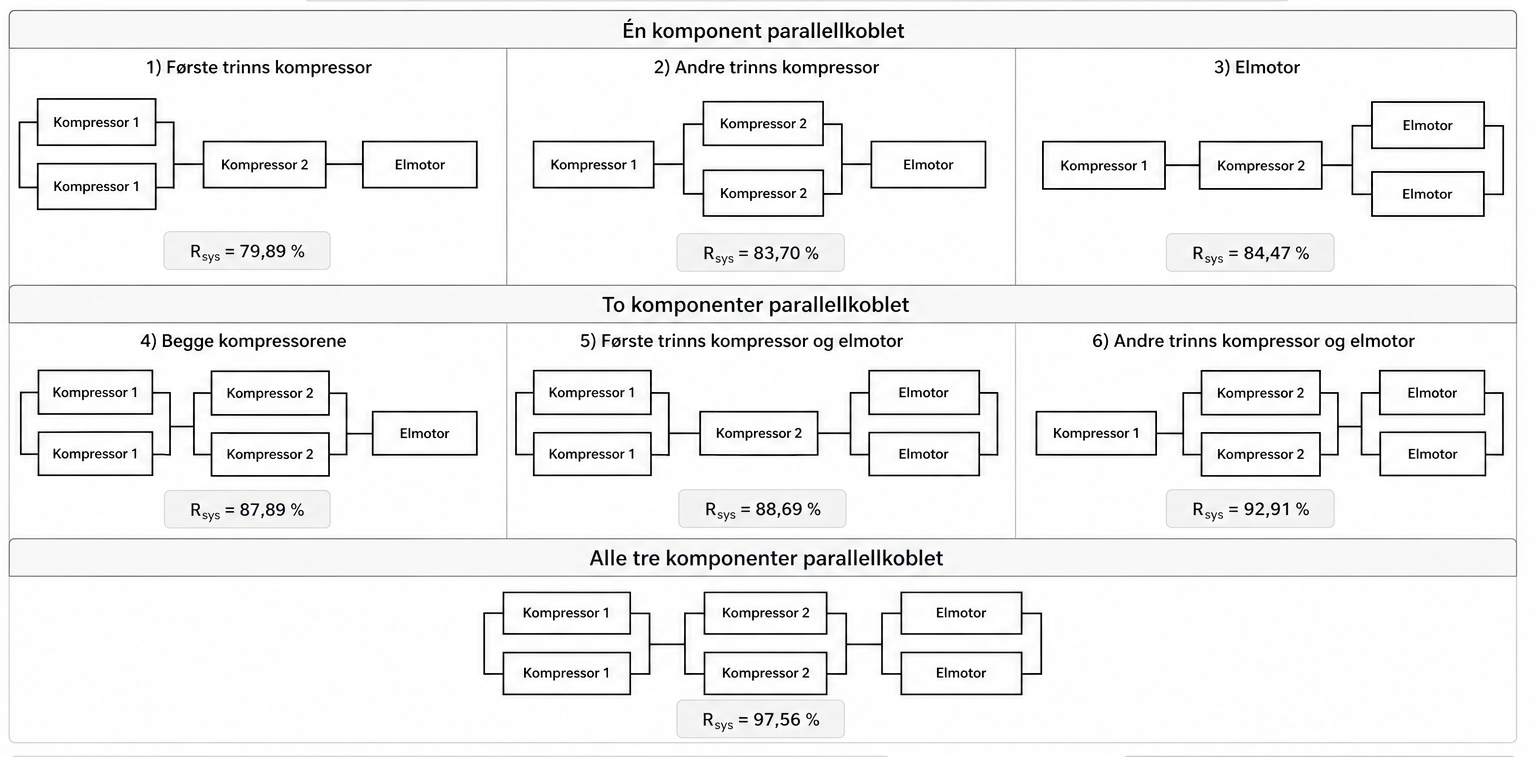
\includegraphics[width=1.0\linewidth]{MAST1102 DV Oppgave 3 Tabell.png}
\caption{Grafisk fremstilling av Tabell 2}
\label{fig:mast1102}
\end{figure}

Avhengig av hvilke komponenter som parallellkobles, kan systempåliteligheten økes fra omtrent 80\% til 98\%.

Beregningene forutsetter at redundante komponenter er uavhengige og identiske med de opprinnelige komponentene. I praksis kan dette være en forenkling. På en oljeplattform kan fellesfeil, begrenset plass, økt vekt, økt vedlikeholdsbehov og høy investeringskostnad redusere nytteverdien av redundans. Beregningene er en ren teknisk sammenligning — vi har ikke sett på kostnader.

\section{Diskusjon}

Resultatene viser at systempåliteligheten forbedres mest ved å parallellkoble de minst pålitelige komponentene. Redundans på andretrinns kompressoren og elmotoren gir en økning i pålitelighet fra 76\% til 93\%. En ytterligere parallellkobling av førstetrinns kompressoren gir en økning til omtrent 98\%.

Førstetrinns kompressor har den lengste reparasjonstiden (MTTR = 40 timer). Dersom begge kompressorene får redundans, vil en feil i én kompressor i større grad kunne håndteres uten umiddelbar stans i kompressortoget. Dette kan redusere konsekvensen av de lange reparasjonstidene for kompressorene. Likevel er det ikke beregnet en samlet systemtilgjengelighet i denne rapporten, og MTTR-verdiene bør derfor tolkes som et beslutningsgrunnlag, ikke som direkte system-MTTR.

Her må det vurderes om ønsket pålitelighet, reparasjonstid og andre begrensninger som plass, vekt, investeringskostnad, økt vedlikeholdsbehov og risiko for fellesfeil veier inn på valg av løsning. Tre forslag presenteres:

\textbf{\large Forslag 1 - Full redundans}

Alle tre komponentene parallellkobles. Som tabell~\ref{tab:redundans} viser gir dette høyest pålitelighet, men det krever dobling av alle komponenter. Det må vurderes om plass, vekt og risiko for fellesfeil på plattformen tillater et slikt inngrep.

\textbf{\large Forslag 2 - Prioritere pålitelighet}

Andretrinns kompressoren og elmotoren parallellkobles. Dette gir nest høyest pålitelighet ved bare fem komponenter, og er billigere og lettere enn full redundans. Førstetrinns kompressor har fortsatt MTTR på 40 timer, så en feil der kan gi lengre nedetid.

\textbf{\large Forslag 3 - Prioritere MTTR}

Begge kompressorene parallellkobles. Påliteligheten er lavere enn i forslag 2, men redundansen gjør at en kompressorfeil ikke nødvendigvis stopper toget. Flaskehalsen for reparasjonstid blir da elmotoren med MTTR på bare 4 timer.

\section{Konklusjon}

Systempåliteligheten til kompressortoget kan økes en god del ved parallellkobling av redundante komponenter. Dersom målet utelukkende er høyest systempålitelighet, er full redundans det beste alternativet, med beregnet pålitelighet på 97{,}56\%. Dersom kostnad, plass og vekt vektlegges, fremstår redundans på andretrinns kompressor og elmotor som et mer balansert tiltak, siden dette øker systempåliteligheten fra 76{,}10\% til 92{,}91\% uten å doble hele kompressortoget. Redundans på begge kompressorene kan være aktuelt dersom hovedmålet er å redusere konsekvensen av lang reparasjonstid, men dette gir lavere beregnet pålitelighet enn alternativet med redundans på andretrinns kompressor og elmotor. Beregningene er basert på idealiserte forutsetninger om uavhengige og identiske komponenter, og en fullstendig vurdering bør også inkludere praktiske begrensninger og økonomiske analyser.


\newpage
\printbibliography[title={Referanser}]

\end{refsection}

% ============================================================
%  OPPGAVE 4: Pelton – virkningsgrad
% ============================================================
\reportstart
\begin{refsection}[Oppgave4/references.bib]

\newpage
\begin{titlepage}
\vbox{ }
\vbox{ }
\begin{center}

\includegraphics[width=0.40\textwidth]{NTNU_logo.png}\\[1cm]
\textsc{\Large MAST1102 - Maskinteknikk 2}\\[0.5cm]
\textsc{\Large Industriell Drift og Vedlikehold}\\[0.5cm]
\vbox{ }
\HRule \\[0.4cm]
{ \huge \bfseries Rapport 4: Pelton – virkningsgrad}\\[0.4cm]
\HRule \\[1.5cm]
\large
\emph{Kandidatnummer:}\\
\vfill
{\large Dato 08/05/2026 }
\end{center}
\end{titlepage}

\frontmatter

\newpage
\section*{Sammendrag}
I denne laboratorierapporten er virkningsgraden til en Pelton-turbin undersøkt ved hjelp av et laboratorieoppsett med lukket vannkretsløp. Målet med forsøket var å analysere hvordan ulike nålposisjoner og belastninger påvirker turbinens ytelse. Forsøket ble gjennomført ved to ulike nålposisjoner, der turtall, dreiemoment, volumstrøm og trykk ble direkte avlest fra oppsettet. Basert på disse måleverdiene ble mekanisk effekt, hydraulisk effekt og virkningsgrad beregnet.

Resultatene viser at nålposisjon 3 ga høyest målt virkningsgrad på 58,4\% mens nålposisjon 7 oppnådde en maksimal virkningsgrad på 50,7\%. For begge nålposisjonene ble maksimal virkningsgrad oppnådd ved tilnærmet samme turbinturtall, noe som samsvarer med teori for Pelton-turbiner. De målte virkningsgradene fremstår rimelige for et lite laboratorieoppsett, men de er lavere enn det som normalt forventes for større, optimaliserte Pelton-turbiner i fullskala drift. Resultatene viser videre at nålposisjonen påvirker nivået på virkningsgraden, og det anbefales å utføre ytterligere målinger med flere nålposisjoner for å fastslå optimal drift.

\newpage
\localtableofcontents
\locallistoffigures
\locallistoftables

\mainmatter

\newpage
\section*{Innledning}
\addcontentsline{toc}{section}{Innledning}

Pelton-turbiner benyttes i vannkraftverk for å omdanne vannets kinetiske energi til mekanisk energi i turbinen, som videre kan omdannes til elektrisk energi ved hjelp av en generator \parencite{Turbiner}. I denne laboratorierapporten analyseres to forsøk med en Pelton-turbin, der turbinens ytelse vurderes under ulike driftsforhold, blant annet som funksjon av vannstrålens påvirkning og den påførte akselbelastningen. Måledata fra forsøket benyttes til å beregne turbinens virkningsgrad. Hensikten med forsøket er å undersøke hvordan ulike driftsinnstillinger påvirker virkningsgraden til Pelton-turbinen.
\section*{Teori}
\setcounter{section}{1}
\setcounter{subsection}{0}
\addcontentsline{toc}{section}{Teori}

\subsection{Pelton-turbin}


En Pelton-turbin er en impulsturbin konstruert for å utnytte vannets tilgjengelige kinetiske energi på en effektiv måte. Slike turbiner benyttes typisk i vannkraftverk med høyt fall relativt lav vannføring, der energien i vannstrålen omdannes til mekanisk rotasjonsenergi i løpehjulet \parencite{Turbiner}.
Vannets hastighet reguleres ved hjelp av en dyse, der trykkenergien i vannet omdannes til kinetisk energi. Ved økt trykfall over dysen vil utløpshastigheten øke, gitt konstant massestrøm, noe som resulterer i høyere kinetisk energi i vannstrålen \parencite{HM4501_Pelton-Turbine}. Sammenhengen mellom volumstrøm $Q$, tverrsnittsareal $A$ og hastighet $v$ er gitt ved kontinuitetslikningen 
\[
v = \frac{Q}{A}.
\]


I en Pelton-turbin skjer trykkfallet hovedsakelig i dysen/injektoren. Det er her trykkenergien fra vannet omdannes til kinetisk energi i vannstrålen før strålen treffer skovlene på løpehjulet. Selve løpehjulet arbeider derfor hovedsakelig med å endre vannets bevegelsesmengde, ikke med å utnytte et stort trykkfall gjennom turbinen.

Vannstrålen treffer deretter skovlene på turbinens løpehjul, som er utformet for å endre vannets strømningsretning mest mulig. Denne retningsendringen medfører en endring i vannets bevegelsesmengde og dermed en impuls som resulterer i en kraft på skovlene. Denne kraften gir opphav til et dreiemoment som får turbinen til å rotere \parencite{Turbiner}. Bevegelsesmengden til vannet kan uttrykkes som 
\[
p = m \cdot v
\]
mens impulsen er definert som endringen i bevegelsesmengde
\[
I = \Delta p = m\left(v_{ut} - v_{inn}\right).
\]

Løpehjulet er koblet til en aksling som overfører den mekaniske effekten videre til en last. I et virkelig vannkraftverk vil denne lasten typisk være en generator. I lab-oppsettet benyttes et bremsebelte koblet til en bremsetrommel for å påføre og regulere belastningen på akslingen. Bremsemekanismen simulerer dermed generatorbelastningen i et virkelig vannkraftverk. Dreiemomentet som påføres akslingen måles ved hjelp av en ekstern kraftsensor.

\subsection{Virkningsgrad}
Pelton-turbiner benyttes i vannkraftverk for å omdanne vannets energi til mekanisk rotasjonsenergi, som videre kan utnyttes til elektrisitetsproduksjon. Hvor effektivt denne energiomdanningen skjer, beskrives ved turbinens virkningsgrad, som defineres som forholdet mellom avgitt mekanisk effekt og tilført hydraulisk effekt \parencite{Turbiner}.

Virkningsgraden uttrykkes som
\[
\eta_{effekt} = \frac{P_{mekanisk}} {P_{hydraulisk}}.
\]

Den mekaniske effekten på turbinakselen er gitt ved
\[
P_{mekanisk} = 2\pi n  M = \omega  M,
\]
der $n$ er turbinens rotasjonshastighet og $M$ er påført dreiemoment. Den mekaniske effekten representerer den nyttige effekten som er overført fra vannstrålen til turbinens løpehjul.
Den hydrauliske effekten er gitt ved
\[
P_{hydraulisk} = \rho  Q  Y,
\]
der $\rho$ er vannets tetthet, $Q$ er volumstrømmen og $Y$ er den spesifikke energien i vannstrålen. Den spesifikke energien kan uttrykkes som
\[
Y = \frac{1}{\rho}(p_{3}-p_{amb})+\frac{1}{2}C_{i}^2 
\]
og består av både trykkenergi og kinetisk energi. Her er $p_{3}$ trykket målt ved trykksensor $P_{3}$, $p_{amb}$ er atmosfæretrykket, og $C_{i}$ er vannets hastighet før dysen.

Vannhastigheten beregnes ved hjelp av kontinuitetslikningen
\[
C_{i}=\frac{Q}{A_{i}}
\]
der $A_{i} = 0,001029m^2$ er tverrsnittsarealet av røret ved trykksensoren \parencite{HM4501_Pelton-Turbine}.

Virkningsgraden gir dermed et mål på hvor effektivt turbinen utnytter den tilførte hydrauliske energien. Ved å analysere virkningsgraden for ulike driftsforhold kan man identifisere optimal drift og vurdere energitap i systemet.


\section*{Lab-oppsettet}
\setcounter{section}{2}
\addcontentsline{toc}{section}{Lab-oppsettet}

\setcounter{subsection}{0}
\subsection{Lab-oppsettet}

Lab-oppsettet består av et lukket vannkretsløp der en sentrifugalpumpe driver vannet fra tanken og frem til Pelton-turbinen. Vannstrømmen reguleres med en ventil, mens dyseåpningen justeres med nålposisjonen. I forsøket ble nålposisjon 7 og 3 undersøkt.

De viktigste måleverdiene i forsøket var volumstrøm, innløpstrykk til turbinen, turbinturtall og dreiemoment på turbinakselen. Volumstrømmen ble målt med strømningsmåler, trykket ble målt ved turbinens innløp, turtallet ble registrert med turtallssensor, og dreiemomentet ble målt ved hjelp av bremsesystemet og kraftsensoren.

Belastningen på turbinen ble endret ved å stramme bremsereimen rundt bremsetrommelen. Økt belastning gir høyere dreiemoment, men lavere turtall. Dette gjør det mulig å undersøke hvordan virkningsgraden varierer med driftspunktet.

De nummererte komponentene er illustrert i figur \ref{fig:lab}.

\section*{Systemets virkemåte}
\setcounter{section}{3}
\addcontentsline{toc}{section}{Systemets virkemåte}

\setcounter{subsection}{0}

\begin{figure}[H]
    \centering
    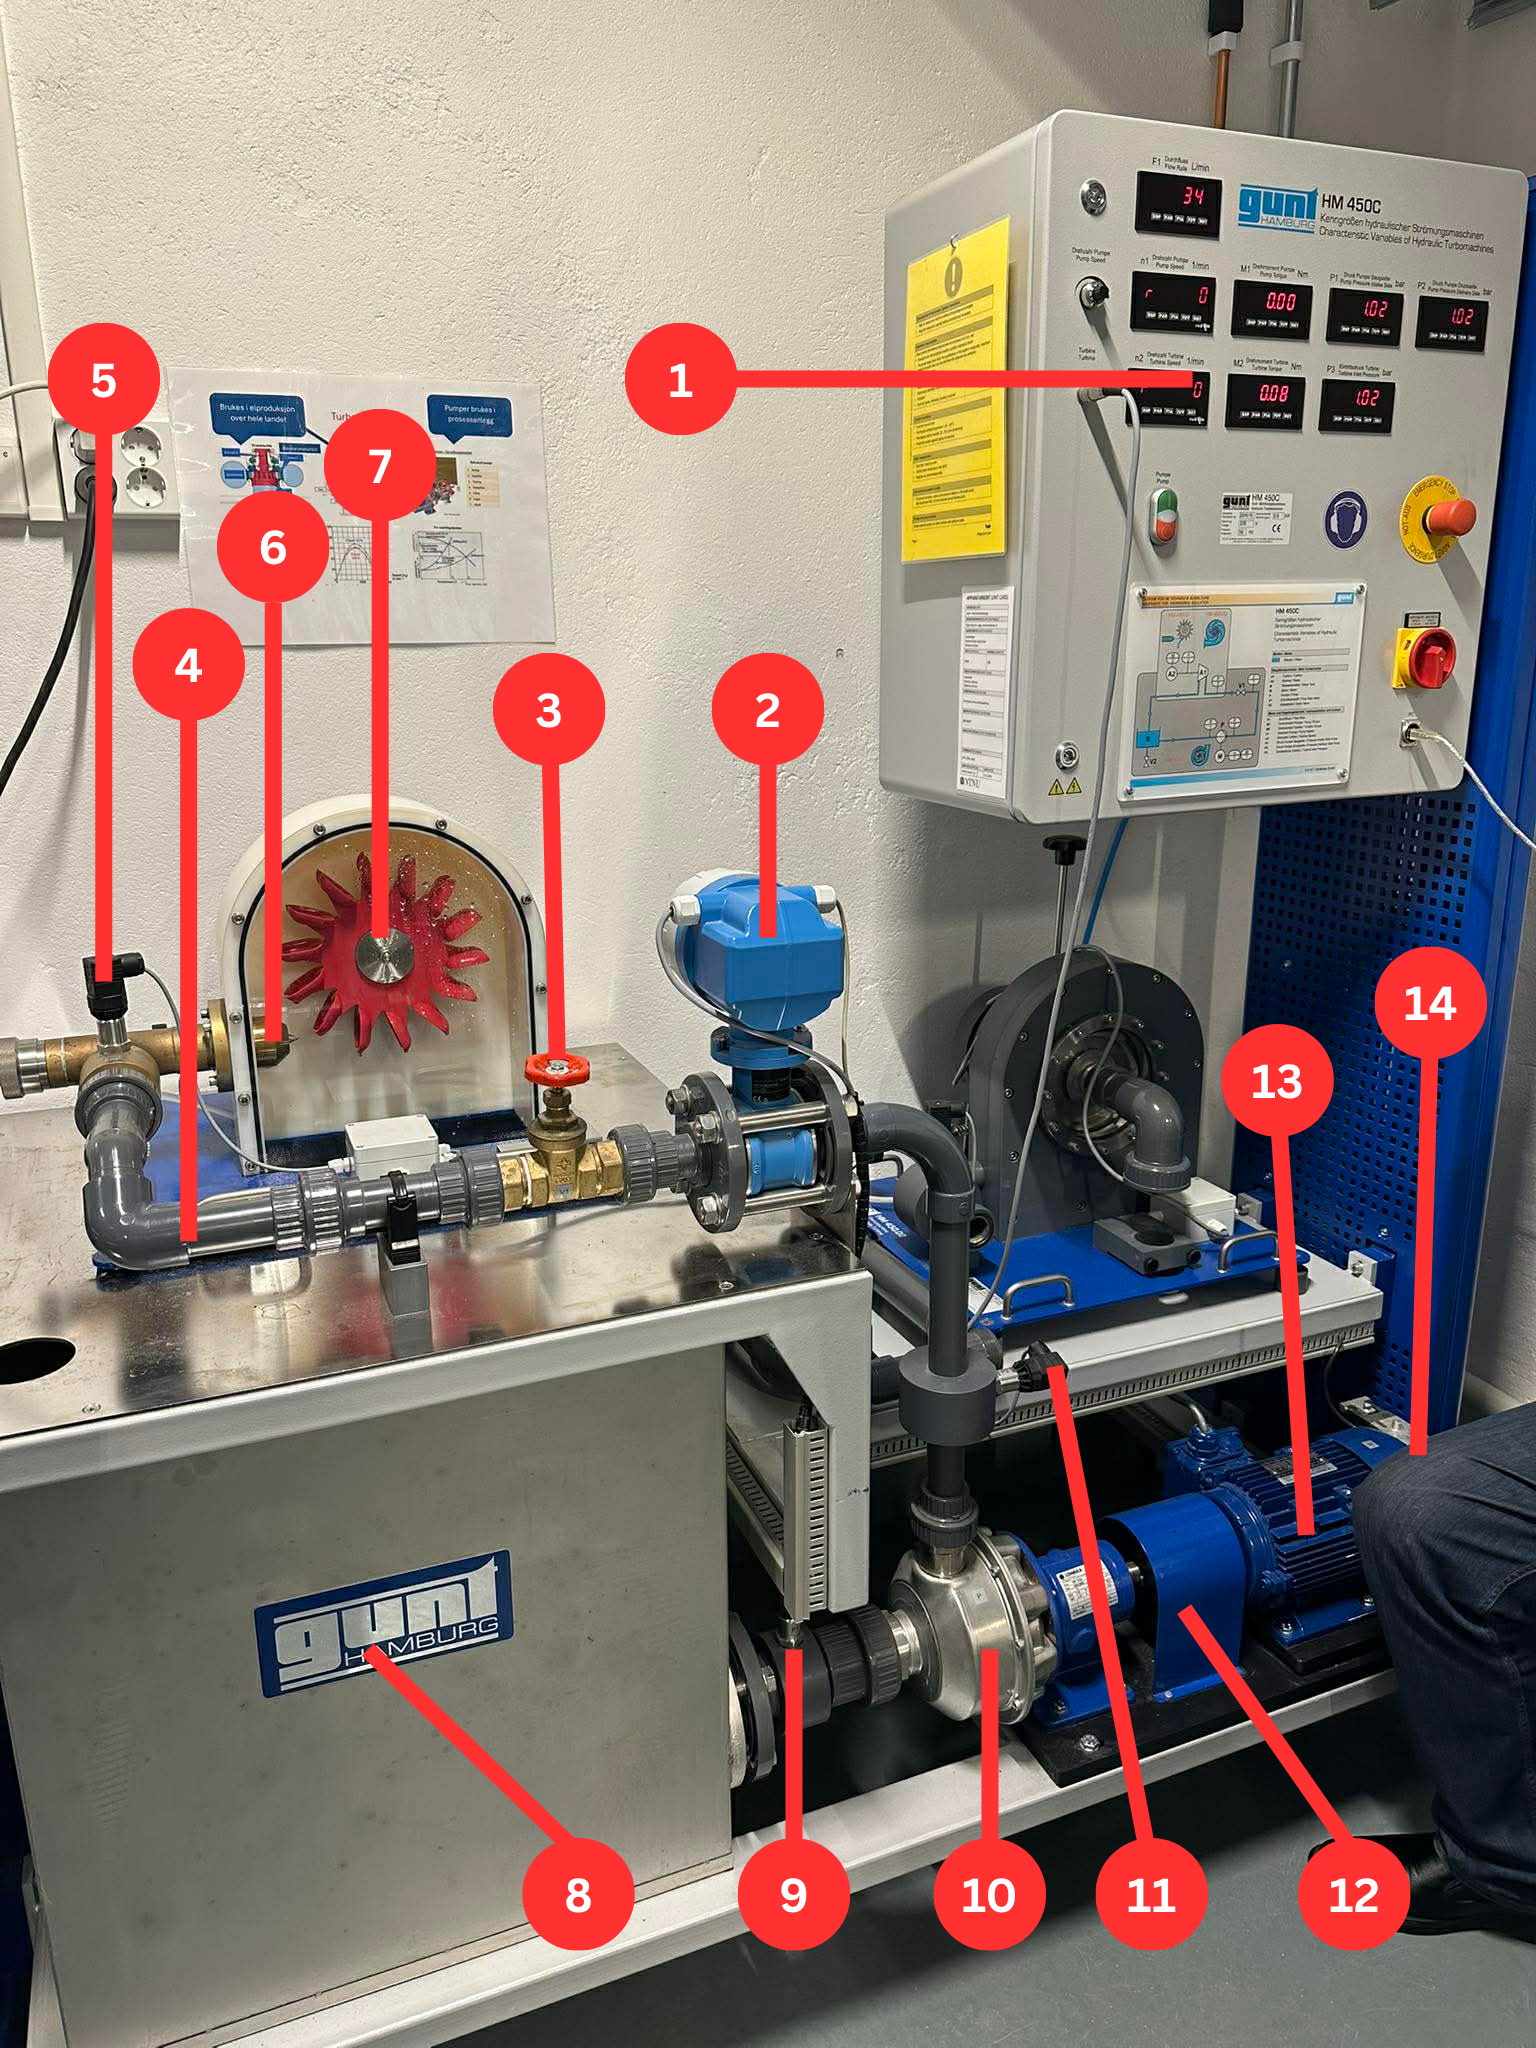
\includegraphics[width=0.5\linewidth]{Ny_lab-oppsett.png}
    \caption{Lab-oppsettet for Pelton-turbin. Nummereringen refererer til hovedkomponentene beskrevet i teksten}
    \label{fig:lab}
\end{figure}


Oppsettet er et lukket vannkretsløp. Pumpen (10) sender vann gjennom tilførselsrøret (4) til dysen (6), som retter en vannstråle mot turbinen (7). Belastningen reguleres med bremsereimen, og turtall, dreiemoment, volumstrøm og trykk avleses direkte fra oppsettet. Etter at vannet har truffet turbinen faller det tilbake til tanken (8), og kretsløpet gjentas.
\section*{Metode}
\setcounter{section}{4}
\addcontentsline{toc}{section}{Metode}

\setcounter{subsection}{0}

Forsøket ble gjennomført ved å undersøke turbinens virkningsgrad for to ulike nålposisjoner. Pumpeturtallet ble først stilt inn til omtrent 2900 rpm. Deretter ble volumstrømmen justert til omtrent 170 L/min for nålposisjon 7 og 115 L/min for nålposisjon 3.

For hver nålposisjon ble belastningen på turbinakselen økt trinnvis ved å stramme bremsereimen. Ved hvert lastpunkt ble turbinens turtall, dreiemoment, volumstrøm og innløpstrykk lest av etter at målingene hadde stabilisert seg. Disse måleverdiene ble brukt til å beregne mekanisk effekt, hydraulisk effekt og virkningsgrad.

Forsøket ble først gjennomført for nålposisjon 7 og deretter gjentatt for nålposisjon 3. Resultatene ble til slutt sammenlignet ved å plotte virkningsgrad som funksjon av turbinturtall.

\section*{Utregning av virkningsgrader}
\setcounter{section}{5}
\addcontentsline{toc}{section}{Utregning av virkningsgrader}

\setcounter{subsection}{0}


\subsection{Utregning av virkningsgrader}
Turtall, dreiemoment, volumstrøm og trykk ble direkte avlest fra lab-oppsettet under forsøket. Basert på disse målte verdiene ble mekanisk effekt, hydraulisk effekt og virkningsgrad beregnet. Pelton-turbinen ble kjørt med en vannstrøm på omtrent 115 $L/min$ (0,00192 $m^3/s$) og 170 $L/min$ (0,00283 $m^3/s$), samt et turtall på om lag 2900 rpm.
Resultatene for nålposisjon 3 er presentert i tabell \ref{tab:pelton}, mens resultatene for nålposisjon 7 er presentert i tabell \ref{tab:pelton2}.

\begin{table}[htbp]
\centering
\caption{Måledata og beregnede verdier for Pelton-turbin. Nålposisjon 3.}
\label{tab:pelton}
\small
\begin{tabular}{
  c
  S[table-format=4.0]
  S[table-format=2.2]
  S[table-format=2.2]
  S[table-format=1.2]
  S[table-format=6.0]
  S[table-format=1.5]
  S[table-format=3.2]
  S[table-format=3.2]
  S[table-format=2.2]
}
\toprule
{\textbf{Måling}} &
{\textbf{$n_{pumpe}$}} &
{\textbf{$n_{pumpe}$}} &
{\textbf{$n_{turbin}$}} &
{\textbf{$M$}} &
{\textbf{$p_3$}} &
{\textbf{$Q$}} &
{\textbf{$P_{hyd}$}} &
{\textbf{$P_{mech}$}} &
{\textbf{$\eta$}} \\
 &
{\small [1/min]} &
{\small [1/s]} &
{\small [1/s]} &
{\small [Nm]} &
{\small [Pa]} &
{\small [m$^3$/s]} &
{\small [W]} &
{\small [W]} &
{\small [\%]} \\
\midrule
1 & 2909 & 48,48 & 24,53 & 0,75 & 314000 & 0,00192 & 413,49 & 115,61 & 27,96 \\
2 & 2909 & 48,48 & 21,87 & 1,34 & 314000 & 0,00192 & 413,49 & 184,11 & 44,52 \\
3 & 2909 & 48,48 & 17,55 & 2,06 & 314000 & 0,00192 & 413,49 & 227,16 & 54,94 \\
4 & 2909 & 48,48 & 14,78 & 2,60 & 314000 & 0,00192 & 413,49 & 241,50 & 58,41 \\
5 & 2909 & 48,48 &  9,67 & 3,30 & 314000 & 0,00192 & 413,49 & 200,43 & 48,47 \\
6 & 2909 & 48,48 &  2,83 & 4,00 & 314000 & 0,00192 & 413,49 &  71,21 & 17,22 \\
7 & 2909 & 48,48 &  0,00 & 4,60 & 314000 & 0,00192 & 413,49 &   0,00 &  0,00 \\
\bottomrule
\end{tabular}
\end{table}

%%%%%%%%%%%%%%%%%% Tabell 2 %%%%%%%%%%%%%%%%%%%%%%%%%

\begin{table}[htbp]
\centering
\caption{Måledata og beregnede verdier for Pelton-turbin. Nålposisjon 7.}
\label{tab:pelton2}
\small
\begin{tabular}{
  c
  S[table-format=4.0]
  S[table-format=2.2]
  S[table-format=2.2]
  S[table-format=1.2]
  S[table-format=6.0]
  S[table-format=1.5]
  S[table-format=3.2]
  S[table-format=3.2]
  S[table-format=2.2]
}
\toprule
{\textbf{Måling}} &
{\textbf{$n_{pumpe}$}} &
{\textbf{$n_{pumpe}$}} &
{\textbf{$n_{turbin}$}} &
{\textbf{$M$}} &
{\textbf{$p_3$}} &
{\textbf{$Q$}} &
{\textbf{$P_{hyd}$}} &
{\textbf{$P_{mech}$}} &
{\textbf{$\eta$}} \\
 &
{\small [1/min]} &
{\small [1/s]} &
{\small [1/s]} &
{\small [Nm]} &
{\small [Pa]} &
{\small [m$^3$/s]} &
{\small [W]} &
{\small [W]} &
{\small [\%]} \\
\midrule
1 & 2899 & 48,32 & 22,03 & 0,75 & 263000 & 0,00283 & 472,57 & 103,83 & 21,97 \\
2 & 2899 & 48,32 & 20,07 & 1,34 & 263000 & 0,00283 & 472,57 & 168,95 & 35,75 \\
3 & 2899 & 48,32 & 17,00 & 2,06 & 263000 & 0,00283 & 472,57 & 220,04 & 46,56 \\
4 & 2899 & 48,32 & 14,67 & 2,60 & 263000 & 0,00283 & 472,57 & 239,60 & 50,70 \\
5 & 2899 & 48,32 & 11,50 & 3,30 & 263000 & 0,00283 & 472,57 & 238,45 & 50,46 \\
6 & 2899 & 48,32 &  7,83 & 4,00 & 263000 & 0,00283 & 472,57 & 196,87 & 41,66 \\
7 & 2899 & 48,32 &  3,33 & 4,60 & 263000 & 0,00283 & 472,57 &  96,34 & 20,39 \\
8 & 2899 & 48,32 &  0,00 & 5,30 & 263000 & 0,00283 & 472,57 &   0,00 &  0,00 \\
\bottomrule
\end{tabular}
\end{table}



%%%%%%%%%%%%%%%%%%% Graf %%%%%%%%%%%%%%%%%%%%%%%%%%

\begin{figure}[H]
\centering
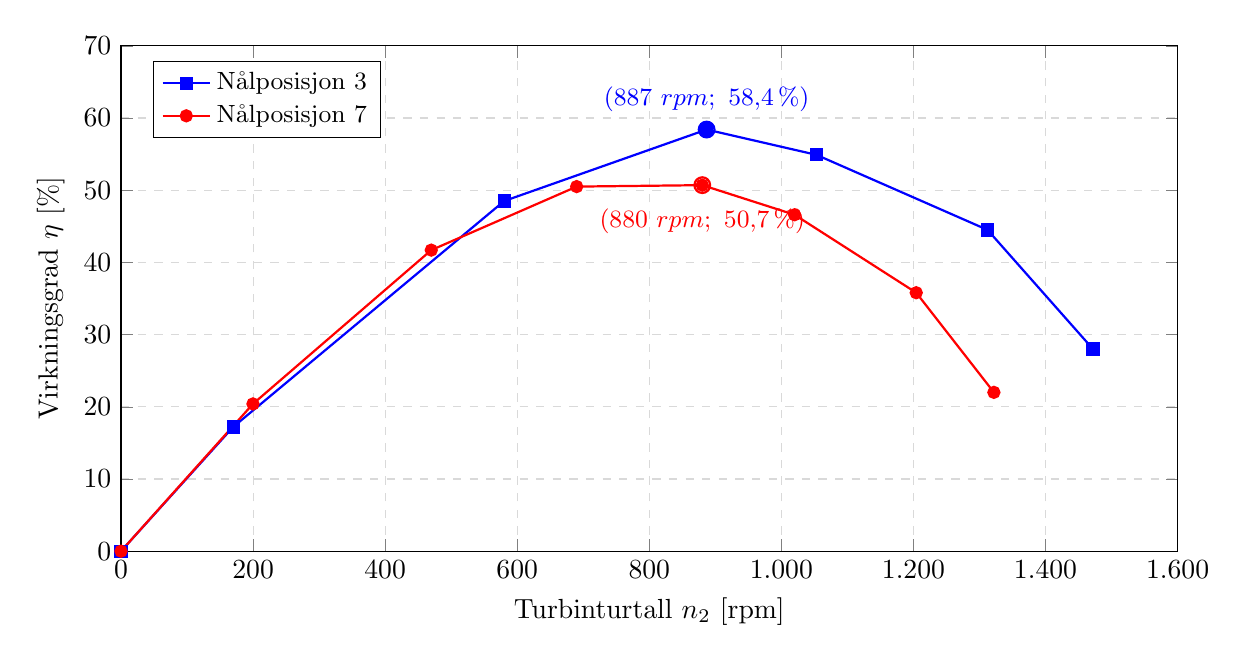
\begin{tikzpicture}
\begin{axis}[
    width=15cm,
    height=8cm,
    xlabel={Turbinturtall $n_2$ [rpm]},
    ylabel={Virkningsgrad $\eta$ [\%]},
    xmin=0, xmax=1600,
    ymin=0, ymax=70,
    grid=major,
    grid style={dashed, gray!30},
    legend pos=north west,
    legend style={font=\small},
    tick label style={/pgf/number format/use comma},
    every axis plot/.append style={thick},
]

\addplot[color=blue, mark=square*, mark size=2pt] coordinates {
    (0,  0.0)
    (169.8, 17.2)
    (580.2, 48.5)
    (886.8, 58.4)
    (1053.0, 54.9)
    (1312.2, 44.5)
    (1471.8, 28.0)
};
\addlegendentry{Nålposisjon 3}

\addplot[color=red, mark=*, mark size=2pt] coordinates {
    (0,  0.0)
    (199.8, 20.4)
    (469.8, 41.7)
    (690.0, 50.5)
    (880.2, 50.7)
    (1020.0, 46.6)
    (1204.2, 35.8)
    (1321.8, 22.0)
};
\addlegendentry{Nålposisjon 7}

% Toppunkt nålposisjon 3
\node[circle, draw=blue, inner sep=2pt, thick] at (axis cs:886.8, 58.4) {};
\node[anchor=south, blue, font=\small]
    at (axis cs:886.8, 59.5) {$(887\ \text{rpm};\ 58{,}4\,\%)$};

% Toppunkt nålposisjon 7
\node[circle, draw=red, inner sep=2pt, thick] at (axis cs:880.2, 50.7) {};
\node[anchor=north, red, font=\small]
    at (axis cs:880.2, 48.8) {$(880\ \text{rpm};\ 50{,}7\,\%)$};

\end{axis}
\end{tikzpicture}
\caption{Virkningsgrad som funksjon av turbinturtall for to nålposisjoner. Toppunktene er markert.}
\label{fig:virkningsgrad}
\end{figure}

\subsection{Diskusjon}
Maksimal virkningsgrad for nålposisjon 3 ble målt til 58,4\% ved et turtall på 14,78 omdreininger per sekund (887 rpm), mens nålposisjon 7 oppnådde en maksimal virkningsgrad på 50,7\% ved 14,67 omdreininger per sekund (880 rpm). Av de to nålposisjonene, presterte nålposisjon 3 bedre i henhold til maksimal utnyttelse av virkningsgrad.

At nålposisjon 3 gir høyere maksimal virkningsgrad enn nålposisjon 7, tyder på at den lavere vannføringen ved nålposisjon 3 ga et mer gunstig driftspunkt for turbinen. Ved nålposisjon 7 er dyseåpningen større, og volumstrømmen blir høyere. Dette gir større hydraulisk effekt inn i systemet, men resultatene viser at turbinen ikke klarte å omdanne denne ekstra tilførte effekten like effektivt til mekanisk effekt på akselen. Mulige årsaker er større strømnings- og spruttap, mindre optimal treffvinkel mot skovlene eller økte tap i bremsesystemet ved høyere vannføring.

De målte virkningsgradene fremstår rimelige for et lite laboratorieoppsett, men de er lavere enn det som normalt forventes for større, optimaliserte Pelton-turbiner i fullskala drift.

For begge nålposisjonene øker virkningsgraden først når belastningen på turbinen økes. Ved lav belastning er dreiemomentet lavt, og den mekaniske effekten på akselen blir derfor liten selv om turtallet er høyt. Når belastningen økes, øker dreiemomentet, og turbinen klarer å hente ut en større del av den hydrauliske effekten fra vannstrålen. Etter et visst punkt faller virkningsgraden igjen fordi belastningen blir så høy at turtallet reduseres betydelig. Da reduseres den mekaniske effekten, selv om dreiemomentet fortsatt er høyt. Dette forklarer hvorfor virkningsgraden får et tydelig maksimum.

Det ble ikke gjennomført målinger for alle tilgjengelige nålposisjoner, så vi kan ikke fastslå hvilken innstilling som gir best resultat totalt sett.

\subsection{Usikkerhetsvurdering}

Resultatene må vurderes med noe usikkerhet. Momentmålingen var sensitiv og kunne variere før systemet stabiliserte seg. Små avlesningsfeil i dreiemoment og turtall får direkte betydning for beregnet mekanisk effekt. I tillegg ble bare to nålposisjoner undersøkt, slik at forsøket ikke kan fastslå hvilken innstilling som faktisk gir høyest virkningsgrad. Resultatene viser derfor bare hvilken av de to undersøkte innstillingene som ga best ytelse.

\newpage
\section*{Konklusjon}
\addcontentsline{toc}{section}{Konklusjon}

Forsøket undersøkte virkningsgraden til en Pelton-turbin ved to ulike nålposisjoner. Den høyeste målte virkningsgraden ble funnet ved nålposisjon 3, med 58,4\% ved et turbinturtall på 14,78 $s^{-1}$, tilsvarende omtrent 887 rpm. For nålposisjon 7 var maksimal virkningsgrad 50,7\% ved 14,67 $s^{-1}$, tilsvarende omtrent 880 rpm.

Resultatene viser at nålposisjonen påvirker hvor effektivt turbinen omdanner hydraulisk effekt til mekanisk effekt. Selv om nålposisjon 7 ga høyere volumstrøm og større hydraulisk effekt, ga den lavere maksimal virkningsgrad enn nålposisjon 3. Dette tyder på at nålposisjon 3 ga et mer gunstig driftspunkt i dette forsøket.

Siden bare to nålposisjoner ble undersøkt, kan forsøket ikke fastslå den optimale innstillingen for turbinen. For å gjøre dette mer presist bør flere nålposisjoner testes, og målingene bør gjentas for å redusere usikkerheten.


\newpage
\printbibliography[title={Referanser}]

\end{refsection}

% ============================================================
%  OPPGAVE 5: Refleksjonsoppgave
% ============================================================
\reportstart
\begin{refsection}[Oppgave5/references.bib]

\newpage
\begin{titlepage}
\vbox{ }
\vbox{ }
\begin{center}

\includegraphics[width=0.40\textwidth]{NTNU_logo.png}\\[1cm]
\textsc{\Large MAST1102 - Maskinteknikk 2}\\[0.5cm]
\textsc{\Large Industriell Drift og Vedlikehold}\\[0.5cm]
\vbox{ }
\HRule \\[0.4cm]
{ \huge \bfseries Rapport 5: Refleksjonsoppgave}\\[0.4cm]
\HRule \\[1.5cm]
\large
\emph{Kandidatnummer:}\\
\vfill
{\large Dato: 08/05/2026 }
\end{center}
\end{titlepage}

\frontmatter

\newpage
\localtableofcontents

\mainmatter

\newpage
\deloppgave{Deloppgave 5.1 -- IDV i næringslivet}
\section*{Introduksjon}
\addcontentsline{toc}{section}{Introduksjon}
Drift og vedlikehold havner ofte i bakgrunnen sammenlignet med design og produksjon, men er i praksis avgjørende for at tekniske systemer skal fungere pålitelig, sikkert og lønnsomt over tid. Før dette emnet forbandt vi vedlikehold mest med reparasjon etter feil. Gjennom arbeidet med oppgaven ser vi at vedlikehold i større grad handler om risikostyring, levetidskostnader og beslutninger basert på data. I dette notatet ser vi på hvorfor kompetanse innen drift og vedlikehold er viktig, hvordan den brukes i vannkraftsektoren, og hvordan vi tror feltet vil utvikle seg det neste tiåret.

\section*{Hvorfor drift og vedlikehold er viktig}
\addcontentsline{toc}{section}{Hvorfor drift og vedlikehold er viktig}

\subsection*{Sikkerhet}
\addcontentsline{toc}{subsection}{Sikkerhet}
Den viktigste rollen til drift og vedlikehold er å opprettholde sikkerheten til utstyret som brukes, enten det er en bro, en heis eller en maskin i en fabrikk. Ved å ha kontroll på tilstanden til utstyret kan man hindre ulykker som følge av slitasje og lignende feil. For å jobbe systematisk med dette brukes metoder som pålitelighetssentrert vedlikehold (RCM) \parencite{saeja1011} og feilmodus- og effektanalyse (FMEA) \parencite{iec60812}. Disse kartlegger hvordan komponenter kan svikte og hvilke konsekvenser det kan få, slik at vedlikeholdsinnsatsen kan prioriteres der risikoen er størst.

I kritisk infrastruktur som vannkraftverk og offshore-installasjoner kan konsekvensene av svikt være alvorlige, ikke bare for bedriften, men for samfunnet. Vedlikehold er derfor regulert gjennom lovverk som internkontrollforskriften \parencite{internkontrollforskriften}, som stiller krav til systematisk HMS-arbeid. God vedlikeholdspraksis er dermed ikke bare et spørsmål om lønnsomhet, men et lovpålagt ansvar.

\subsection*{Økonomi}
\addcontentsline{toc}{subsection}{Økonomi}
Drift og vedlikeholdsingeniører kan analysere hvordan pålitelighet, reparasjonstid og flaskehalser påvirker produksjonskapasitet og kostnader. Ved å ha fokus på drift og vedlikehold kan man gjøre et informert valg om hvilken produksjonsmetode man skal bruke og hvordan produksjonen bør settes opp.

I en fabrikk er det som regel en form for løpebåndproduksjon. Hvert steg er avhengig av at det forrige er utført, så en stopp i én del av fabrikken kan fort gå utover hele linja. En drift og vedlikeholdsingeniør kan regne seg frem til påliteligheten til de forskjellige produksjonsstegene, og til linja som helhet. Da ser man om fabrikken utnytter kapasiteten godt, og om det bør legges inn redundans i enkelte steg basert på pålitelighet og reparasjonstid. Gode vurderinger minimerer nedetid og øker dermed fortjenesten.

Også i offentlig forvaltning spiller vedlikehold en viktig økonomisk rolle. Kommuner og stat forvalter store verdier i form av veier, broer, vannforsyning og bygninger. Utsatt vedlikehold kan se ut som en innsparing på kort sikt, men fører ofte til at skader vokser og reparasjonskostnadene blir langt høyere enn de hadde trengt å være. Et levetidskostnadsperspektiv, der man ser på totalkostnaden over utstyrets levetid, gir som regel et bedre grunnlag for beslutninger enn å bare se på årets budsjett.

\subsection*{Bærekraft og miljø}
\addcontentsline{toc}{subsection}{Bærekraft og miljø}
Ved hjelp av tilstandsovervåking kan en drift og vedlikeholdsingeniør vurdere den faktiske tilstanden til en maskin og bestemme når komponenter bør skiftes ut. Med moderne tilstandsovervåking kan man planlegge vedlikeholdet slik at man tar så mye som mulig samtidig, i stedet for å bytte deler etter faste intervaller eller vente til noe havarerer. Dette forlenger levetiden til utstyret og reduserer behovet for å produsere nye deler. Mindre produksjon betyr lavere energiforbruk, mindre råvareutvinning og mindre avfall. I tillegg reduserer godt vedlikehold risikoen for akutte havarier som kan føre til utslipp av olje, kjemikalier eller andre forurensende stoffer. Godt vedlikehold gjør altså at utstyr varer lenger, færre deler må byttes unødvendig, og risikoen for utslipp ved havari blir lavere.

\section*{Drift og vedlikehold i vannkraftsektoren}
\addcontentsline{toc}{section}{Drift og vedlikehold i vannkraftsektoren}
Vannkraftsektoren er en næring som har stor nytte av kompetanse innen drift og vedlikehold. Vannkraftverk er en viktig del av samfunnets infrastruktur, og god drift sikrer en pålitelig og lønnsom produksjon av elektrisk energi.

\subsection*{Pålitelighet og tilgjengelighet}
\addcontentsline{toc}{subsection}{Pålitelighet og tilgjengelighet}
Pålitelighet handler om anleggets evne til å levere energi stabilt over tid. Tilgjengelighet handler om hvor stor andel av tiden anlegget er operativt og klart til bruk. Begge påvirkes direkte av vedlikeholdet. Komponenter som turbiner, generatorer og luker må fungere som de skal, dag etter dag. Slitasje på turbinblader eller ledeskovler kan føre til redusert virkningsgrad, og i verste fall til havari som krever langvarig stans. Mangelfullt vedlikehold øker risikoen for uplanlagt driftsstans, mens for hyppig vedlikehold gir unødvendig nedetid. God vedlikeholdsplanlegging handler om å finne balansen.

\subsection*{Tilstandsovervåking og IoT}
\addcontentsline{toc}{subsection}{Tilstandsovervåking og IoT}
Tilstandsovervåking er spesielt viktig i vannkraftverk, der mange komponenter er vanskelig tilgjengelige og kostbare å reparere. En generator som er bygget inn i fjellet kan ikke uten videre inspiseres visuelt, men vibrasjonssensorer kan fange opp endringer som tyder på lagerskade lenge før det blir et problem. Temperaturmålinger på transformatorer og trykkmålinger i vannveiene gir tilsvarende innsikt.

Bruken av IoT har gjort slik overvåking mer tilgjengelig. Ved å installere sensorer på kritiske komponenter kan man samle inn data om vibrasjon, temperatur, trykk og vannføring i sanntid. Disse dataene kan overføres til sentrale systemer der de analyseres og sammenlignes med historiske verdier. Det gjør det mulig å oppdage trender og avvik som ellers ville gått ubemerket hen. Dersom vibrasjonsdata viser økende ubalanse i en turbin, kan vedlikehold planlegges til et tidspunkt med lav kraftpris eller lav etterspørsel, i stedet for at feilen utvikler seg til uplanlagt stans. Slike beslutninger er kjernen i det tilstandsovervåking handler om -- ikke bare å samle data, men å bruke dem til å ta bedre vedlikeholdsbeslutninger.

Økt digitalisering medfører også nye utfordringer. Når sensorer og styringssystemer kobles til nettverk, blir vannkraftverk mer sårbare for cyberangrep. Vannkraft er kritisk infrastruktur, og et angrep kan i verste fall stanse produksjonen eller føre til ukontrollert drift. Digital sikkerhet er derfor en viktig del av driften når slike løsninger tas i bruk.

\section*{Fremtidens drift og vedlikehold}
\addcontentsline{toc}{section}{Fremtidens drift og vedlikehold}

Drift og vedlikehold av teknisk utstyr er i ferd med å gjennomgå en stor endring, drevet av det som ofte kalles den fjerde industrielle revolusjon (Industri 4.0) \parencite{schwab2016}. Den første revolusjonen handlet om dampkraft. Den andre industrielle revolusjonen forbindes med masseproduksjon, slik Chaplins \textit{Modern Times} karikerer gjennom bildet av mennesket som et tannhjul i maskineriet. Den tredje revolusjonen handlet i større grad om datamaskiner og automasjon. Den fjerde kjennetegnes av at fysiske systemer kobles tett sammen med digitale gjennom sensorer, nettverk og kunstig intelligens. Om ti år tror vi at vedlikehold vil ha gått fra å være en planlagt eller reaktiv aktivitet til en kontinuerlig, datadrevet prosess hvor utstyret i stor grad varsler om sin egen tilstand.

En viktig trend er prediktivt vedlikehold (Predictive Maintenance). I stedet for å bytte komponenter etter faste intervaller eller vente til noe havarerer, vil maskiner være utstyrt med sensorer som måler vibrasjon, temperatur, strømtrekk, akustikk og oljekvalitet i sanntid. Disse dataene mates inn i maskinlæringsmodeller som kan oppdage mønstre som indikerer begynnende slitasje -- for eksempel at et lager nærmer seg utmatningsbrudd flere uker før det faktisk svikter. Dette reduserer både uplanlagt nedetid og unødvendige komponentbytter, og er kjernen i konseptet Smart Vedlikehold.

Tett knyttet til dette er digitale tvillinger (Digital Twins). En digital tvilling er en virtuell kopi av et fysisk system, for eksempel en pumpe, en vindturbin eller en hel produksjonslinje, som kontinuerlig oppdateres med driftsdata fra det virkelige utstyret. Vedlikeholdsingeniører kan kjøre simuleringer på tvillingen for å forutsi hvordan endringer i belastning eller driftsforhold vil påvirke levetid og ytelse, uten å risikere det fysiske anlegget. Kombinert med skytjenester og edge computing gjør dette det mulig å overvåke store, geografisk spredte anlegg fra et sentralt kontrollrom.

På verkstedgulvet vil utvidet virkelighet (AR) og autonome systemer trolig spille en stadig større rolle. En tekniker med AR-briller kan få instruksjoner, måleverdier og 3D-modeller lagt over synsfeltet mens hen jobber. Samtidig vil droner og inspeksjonsroboter overta farlige eller utilgjengelige inspeksjoner, som visuell inspeksjon av offshore-konstruksjoner eller trykktanker. Dette er et tydelig brudd med \textit{Modern Times}-bildet av mennesket som maskinens forlengelse. I Industri 4.0 er ambisjonen at teknologi skal forsterke menneskelig kompetanse, slik at vedlikeholdspersonell flyttes fra rutinearbeid til analyse og problemløsning.

Om ti år tror vi vedlikehold i større grad vil handle om å tolke data før feil oppstår, ikke bare om å utføre planlagte kontroller eller reparere havarier. Skillet mellom drift, vedlikehold og produktutvikling vil gradvis viskes ut etter hvert som data fra felt mates tilbake til konstruksjons- og forbedringsarbeid.

\section*{Konklusjon}
\addcontentsline{toc}{section}{Konklusjon}
Drift og vedlikehold handler om mer enn å reparere det som går i stykker. Det er en disiplin som påvirker pålitelighet, lønnsomhet, sikkerhet og bærekraft i de fleste tekniske virksomheter. Vannkraftsektoren viser hvordan tilstandsovervåking og IoT allerede i dag gjør det mulig å ta bedre vedlikeholdsbeslutninger, samtidig som det stiller nye krav til digital sikkerhet. Ser vi ti år frem, peker trender som prediktivt vedlikehold, digitale tvillinger og AR mot et fagfelt som blir stadig mer datadrevet. Arbeidet med dette notatet har gjort det tydeligere for oss at drift og vedlikehold ikke er et smalt spesialfelt, men en kompetanse som griper inn i de fleste tekniske virksomheter. Det har styrket vår motivasjon for studieretningen.

\newpage
\deloppgave{Deloppgave 5.2 -- Studier og muligheter}
\setcounter{section}{0}

\section*{Introduksjon}
\addcontentsline{toc}{section}{Introduksjon}
Maskiningeniør er et bredt studium, og drift og vedlikehold er en sentral del av det. I løpet av dette semesteret har vi lært mye om hva drift og vedlikehold innebærer og hvordan undervisningen er lagt opp. Vi har også fått innblikk i arbeidshverdagen til en drift og vedlikeholdsingeniør og mulighetene etter bachelorstudiet. I denne refleksjonen diskuterer vi hva som motiverer oss til å velge studieretning drift og vedlikehold, og hvor viktig kombinasjonen av teori og praksis er for valget.

\section*{Motivasjon}
\addcontentsline{toc}{section}{Motivasjon}

Når man skal velge studieretning, er motivasjon en viktig faktor. Vår motivasjon for å velge drift og vedlikehold bygger på flere ulike inntrykk og erfaringer. Gjennom bedriftsbesøk og innsikt fra tidligere studenter har vi fått et bedre bilde av hva vedlikehold innebærer og hvilke muligheter studiet gir.

Det faglige innholdet i studieretningen er en viktig motivasjonsfaktor. Drift og vedlikehold kombinerer teknisk forståelse av maskiner og systemer med analytiske metoder som pålitelighetsberegning og tilstandsovervåking. Det er et fag der man må forstå hvordan ting fungerer, hvorfor de svikter og hva man kan gjøre for å forhindre det. Denne koblingen mellom teori og praktisk problemløsning er noe vi i gruppen synes er interessant. Før emnet hadde vi et nokså vagt bilde av hva en vedlikeholdsingeniør gjør. Nå ser vi at faget i stor grad handler om å ta beslutninger basert på data og analyse, ikke bare å skifte deler.

Vedlikehold åpner for mange muligheter i arbeidslivet og er etterspurt i flere bransjer, blant annet industri, energi, offshore og produksjon. For vår del virker dette særlig motiverende fordi studieretningen ikke låser oss til én bransje. Den samme kompetansen kan brukes i vannkraft, offshore, produksjon og samferdsel, men med ulike tekniske utfordringer. Fleksibiliteten gir også en trygghet i form av jobbsikkerhet, ettersom vedlikehold er noe det alltid vil være behov for. Det finnes jobbmuligheter både i Norge, fra sør til nord, og internasjonalt.

En annen faktor som motiverer er muligheten for en variert arbeidshverdag. Arbeidshverdagen kan variere mellom planlagt analysearbeid, akutt feilsøking og samarbeid med driftspersonell, noe som gjør fagfeltet mindre ensformig. For oss gjør denne variasjonen fagfeltet mer attraktivt enn en rolle med mer ensidige arbeidsoppgaver.

Studieretningen er godt tilrettelagt for læring. Klassene er relativt små, noe som gir tettere kontakt med foreleserne. RAMS-labben gir tilgang til relevant utstyr for praktiske øvinger, og flere av fagene legger opp til prosjektarbeid i samarbeid med lokal industri. Vi har sett eksempler på at studenter arbeider med reelle problemstillinger for lokale bedrifter. Dette er en fordel når man skal ut i jobb eller finne bacheloroppgave, fordi man allerede har kontakt med bedrifter og kan vise til resultater.

Etter fullført bachelor finnes det gode muligheter for videre studier på masternivå, både i Norge og i utlandet. Ved NTNU på Gløshaugen er det særlig masterprogrammet Maskinteknikk og produksjon (2-årig) som er relevant \parencite{ntnumiprod}. Innen dette programmet kan man velge studieretningen Industriell ledelse og systemfag, med fordypning innen sikkerhet, pålitelighet og vedlikehold. Denne masteren bygger videre på bachelorgraden og gir dypere innsikt i blant annet driftssikkerhet, vedlikeholdsstrategier og analyse av tekniske systemer.

\section*{Kombinasjon av teori og praksis}
\addcontentsline{toc}{section}{Kombinasjon av teori og praksis}
Studieretning drift og vedlikehold er fordelt mellom praktisk arbeid og teori. Labboppgaver gjennomføres i RAMS-labben, og prosjektoppgaver kan ved anledning gjøres i samarbeid med lokal industri.

Hvordan undervisningen er lagt opp har stor påvirkning på hvordan man lærer. Drift og vedlikehold har så langt hatt mye praktisk arbeid. Dette synes vi engasjerer mer enn ren teoretisk læring, fordi man kommer nærmere oppgavene man faktisk vil utføre i arbeidslivet.

Fagene videre i retningen bygger godt på hverandre \parencite{mast2003, mast2004, mast2006, mast2012}. MAST2003 gir grunnlag i kraftoverførende maskindeler og deres tendenser for svikt, mens MAST2004 bruker dette videre i en prosjektoppgave om en reell problemstilling innen drift og vedlikehold. At prosjektoppgaven ligner det man møter i næringslivet gjør den nyttig, ikke bare faglig, men fordi den gir oss en forsmak på hvordan vedlikeholdsproblemer faktisk løses i praksis. MAST2006 dekker analyse av levetid og driftssikkerhet, vedlikeholdsledelse og vedlikeholdsstyringssystemer, mens MAST2012 handler om prediktivt vedlikehold og bruk av tilstandsdata i modeller for prognose og diagnose. Det vi setter mest pris på med disse fagene er at læringsformen -- labøvinger, prosjektarbeid og interaktive forelesninger -- gjør at vi kan prøve ut metodene, ikke bare lese om dem.

\section*{Bacheloroppgaven}
\addcontentsline{toc}{section}{Bacheloroppgaven}
Bacheloroppgaven i sjette semester er en viktig del av studieretningen. Her får man mulighet til å jobbe med en større, reell problemstilling over lengre tid, ofte i samarbeid med en bedrift. Dette skiller seg fra de mindre prosjektoppgavene ved at man må jobbe mer selvstendig og ta ansvar for hele prosessen fra problemdefinisjon til løsningsforslag. Bacheloroppgaven fremstår derfor som et viktig punkt i studieløpet, fordi den gir mulighet til å teste om interessen for praktisk problemløsning og vedlikeholdsanalyse faktisk passer med arbeidsoppgavene i industrien.

\section*{Konklusjon}
\addcontentsline{toc}{section}{Konklusjon}
Drift og vedlikehold er en studieretning som gir kompetanse spisset mot industrien vi vil møte etter endt utdanning. Fagene har god variasjon mellom teori og praksis, noe som gir et solid læringsutbytte. Kombinasjonen av labbarbeid, prosjektoppgaver og bacheloroppgave i samarbeid med bedrifter gjør overgangen til arbeidslivet kortere. Gjennom semesteret har vi gått fra et vagt inntrykk av hva vedlikehold er, til en bedre forståelse av at det handler om systematisk analyse, risikostyring og datadrevne beslutninger. Det har gitt oss et godt grunnlag til å velge veien videre, enten det blir en mastergrad eller rett ut i jobb.


\newpage
\printbibliography[title={Referanser}]

\end{refsection}

\end{document}
